% !TeX document-id = {6284b349-a8b4-4e21-ba1a-ecfc8e7af9bd}
% !BIB TS-program = biber
% !BIB program = biber

\documentclass[11pt]{report}
\usepackage{setspace}
%\usepackage{subfigure}

\def \thesistitle {Multitask \& Meta Learning for Language Models}

\usepackage{amssymb,graphicx,color}
\usepackage{amsfonts}
\usepackage{latexsym}
\usepackage{a4wide}
\usepackage{amsmath}
\usepackage{hyperref}
\usepackage{caption}
\usepackage[svgnames]{xcolor}   
\usepackage{varwidth}
\usepackage{adjustbox}
\DeclareCaptionFormat{myformat}{%
	% #1: label (e.g. "Table 1")
	% #2: separator (e.g. ": ")
	% #3: caption text
	\begin{varwidth}{\linewidth}%
		\centering
		#1#2#3%
	\end{varwidth}%
}
\captionsetup{format=myformat}
\counterwithout*{footnote}{chapter} % Ensure that footnote numbers stay consistent and increase across chapters

\usepackage[a4paper,width=150mm,top=25mm,bottom=25mm,bindingoffset=6mm]{geometry}

\usepackage{multirow}% http://ctan.org/pkg/multirow
\usepackage{booktabs}% http://ctan.org/pkg/booktabs
\usepackage{enumerate}
\usepackage{pdfpages}
\usepackage{algorithm,algorithmicx}
\usepackage[noend]{algpseudocode}
\newcommand*\Let[2]{\State #1 $\gets$ #2}
\usepackage[normalem]{ulem} %Striking through text
% HEADERS
\usepackage{fancyhdr}
\pagestyle{fancy}
\fancyhf{}
\fancyhead[L]{\slshape\nouppercase{\leftmark}}
\fancyhead[R]{\slshape\nouppercase{\thesistitle}}
\renewcommand{\headrulewidth}{0.4pt}
\fancyfoot[C]{\thepage}

% NOMENCLATURE
\usepackage[intoc, english]{nomencl}
\makenomenclature
\renewcommand{\nomname}{List of Common Terms and Symbols}
\renewcommand{\nompreamble}{This list outlines several symbols used frequently and consistently during this thesis.}
\setlength{\nomlabelwidth}{1.5cm}

%% This code creates the groups in the nomenclature
% -----------------------------------------
\usepackage{ifthen}
%\renewcommand\nomgroup[1]{%
%	\item[\bfseries
%	\ifstrequal{#1}{G}{General}{%
%	\ifstrequal{#1}{LM}{Language Modelling}{%
%	\ifstrequal{#1}{Multitask}{Multitask Learning}{%
%	\ifstrequal{#1}{Meta}{Meta Learning}{}}}}%
%	]}
\usepackage{etoolbox}
\renewcommand\nomgroup[1]{%
	\item[\bfseries
	\ifstrequal{#1}{G}{General}{%
		\ifstrequal{#1}{L}{Language Modelling}{%
			\ifstrequal{#1}{M}{Multitask Learning}{%
				\ifstrequal{#1}{Z}{Meta Learning}{}}}}%
	]}
% -----------------------------------------

% BIBTEX
\usepackage[backend=biber, style=numeric, sorting=none]{biblatex}
\addbibresource{BibTeX/MScThesis.bib}
\defbibheading{secbib}[\bibname]{%
	\section*{#1}%
	\markboth{#1}{#1}}

% TIKZ
\usepackage{tikz}
\usepackage{tikzsymbols}
% Save some symbols we want to use as they intefere with the other packages
\newsavebox\Abox
\savebox\Abox{\Smiley[2]}
\def\Smiley{\usebox\Abox}
\newsavebox\Bbox
\savebox\Bbox{\Neutrey[2]}
\def\Neutrey{\usebox\Bbox}
\newsavebox\Cbox
\savebox\Cbox{\Sadey[2]}
\def\Sadey{\usebox\Cbox}
\newsavebox\Dbox
\savebox\Dbox{\Vomey[4.5][green!80!black][olive]}
\def\Chunny{\usebox\Dbox}
\newsavebox\Ebox
\savebox\Ebox{\dCooley[-5][cyan]}
\def\Cooley{\usebox\Ebox}


\usetikzlibrary{matrix, arrows, shapes}
\tikzset{ 
	table/.style={
		matrix of nodes,
		row sep=-\pgflinewidth,
		column sep=-\pgflinewidth,
		nodes={rectangle, align=center, text centered},
		align=center, 
		text centered,
		text depth=4ex,
		text height=2.5ex,
		nodes in empty cells
	},
	row 1/.style={nodes={fill=green!10,text depth=0.4ex,text height=2ex}},
	column 1/.style={nodes={fill=green!10, text width=20ex}},
	column 2/.style={nodes={text width=70ex}},
}
\tikzset{log/.style={rectangle, draw, fill=black, text width=5em, text centered, rounded corners, minimum height=4em}}
\tikzset{boldtext/.style={fill=LemonChiffon, font=\bfseries}}
\tikzset{aspect/.style={circle, draw, fill=green!10, text width=5em, text centered, minimum height=4em}}
\tikzset{sentiment/.style={circle, draw, fill=blue!10, text width=5.5em, text centered, minimum height=1em}}



% MATHS
%\newtheorem{theorem}{THEOREM}
%\newtheorem{lemma}[theorem]{LEMMA}
%\newtheorem{corollary}[theorem]{COROLLARY}
%\newtheorem{proposition}[theorem]{PROPOSITION}
%\newtheorem{remark}[theorem]{REMARK}
%\newtheorem{definition}[theorem]{DEFINITION}
%\newtheorem{fact}[theorem]{FACT}
%
%\newtheorem{problem}[theorem]{PROBLEM}
%\newtheorem{exercise}[theorem]{EXERCISE}
\usepackage{amsthm}
\theoremstyle{Definition}
\newtheorem{theorem}{theorem}[section]
\newtheorem{lemma}[theorem]{Lemma}
\newtheorem{prop}[theorem]{Proposition}
\newtheorem*{cor}{Corollary}
\newtheorem{definition}{Definition}[section]
\newtheorem{conj}{Conjecture}[section]
\newtheorem{example}{Example}[section]

\theoremstyle{remark}
\newtheorem*{remark}{Remark}
\newtheorem*{note}{Note}
\def \set#1{\{#1\} }

%\newenvironment{proof}{
%PROOF:
%\begin{quotation}}{
%$\Box$ \end{quotation}}


% COMMAND OVERRIDES
\newcommand{\N}{\mbox{\( \mathbb N \)}}
\newcommand{\Q}{\mbox{\(\mathbb Q\)}}
\newcommand{\R}{\mbox{\(\mathbb R\)}}
\newcommand{\Z}{\mbox{\(\mathbb Z\)}}

\renewcommand{\P}{\mbox{\(\mathbb P\)}}

%%%%%%%%%%%%%%%%%%%%%%%%%%

% GRAPHICS PATH
\graphicspath{{images/}{images/background/}{images/methodology/}{images/experiments/}}

% THESIS TITLE
\title{  	{ \includegraphics[scale=.5]{ucl_logo.png}}\\
{{\Huge \thesistitle}}\\
{\large An investigation of optimal multitask schemas and generalisation for the automatic construction of Knowledge Graphs with focus on sentiment}\\
		}
\date{Submission date: 6 September 2019}
\author{Ryan Jenkinson\thanks{
{\bf Disclaimer:}
This report is submitted as part requirement for the Computational Statistics and Machine Learning MSc at UCL. It is substantially the result of my own work except where explicitly indicated in the text. The report may be freely copied and distributed provided the source is explicitly acknowledged}
\\ \\
Computational Statistics and Machine Learning MSc\ \\ \\
Industry Supervisors: Dr Erik Mathiesen, Dr Ryan Garland \\
Academic Supervisors: Prof. David Barber, Yap Pau Ching
}

\begin{document}
\onehalfspacing
\maketitle



% DEDICATION
\null\vspace {\stretch{1}}
\begin{flushright}
	To my parents, for their unwavering support in my ambitions.
\end{flushright}
\vspace{\stretch{2}}\null
\thispagestyle{empty}
\newpage

\chapter*{Acknowledgements}
\pagenumbering{gobble}
Firstly, I'd like to thank the Machine Learning and Data Science team: Erik, Ryan, Sophia, James and Marina at Streetbees, for their continual encouragement and support throughout this thesis, and for adopting me as part of the team throughout the summer. Additional thanks go to Jeunghyun Byun, a fellow MSc student in Machine Learning, for his friendliness. Our discussions and meetings have given me valuable insight, and the emphasis on learning and development has been amazing. Secondly to Stanley, for his diligence and perseverance in helping me run my experiments. Thirdly, I'd like to thank my academic supervisor Yap Pau Ching, for her helpful discussions and keeping me on the right track. Finally, to my parents and family, my friends and long term partner, for their unwavering and continual support in all of my ambitions.

\newpage
% ABSTRACT
\begin{abstract}
In this thesis, we aim to investigate how multitask learning can affect the performance of Language Models on difficult downstream aspect based sentiment analysis tasks. We introduce novel task sampling schemas, and leverage dependent subtask hierarchies to fine tune our model jointly on several related tasks in order to regularise the learned embeddings and enabling them to generalise better to our main task. We report major improvements to the current state-of-the-art metrics, of over 2\% relative increase compared to regular transfer learning in some cases, showcasing the efficacy of these schemes. Furthermore, these schemes perform better than regular multitask learning using a ``round robin" strategy, and the methodology is entirely general meaning it could be applied to a variety of different Natural Language Processing tasks, or indeed to other Machine Learning disciplines such as Computer Vision.

Additionally, we conduct an investigation into how different language models learn, and in particular the importance of how the pretraining methodology can lead to representations which generalise better to complicated downstream tasks. This investigation extends the literature in this space and we find important conclusions that multitask pretraining seems to enable better performance on complicated downstream tasks. This is currently an active topic of research for the field.

In order to generalise to new categories, we propose a novel application of Meta Learning to a Few Shot Text Classification regime, and outline how this could be implemented, drawing on the recent literature.

We provide a fully open sourced, commented and code reviewed library for future research in this ever-changing field of transformers for language modelling, and propose ideas for future work in terms of both immediate extensions and longer term ones.
\end{abstract}
\newpage 

% TABLE OF CONTENTS
\pagenumbering{roman}
\tableofcontents
\newpage \cleardoublepage

% LIST OF OTHER THINGS
\addcontentsline{toc}{chapter}{Tables and Figures}
\addcontentsline{toc}{section}{List of Tables}
\pagenumbering{arabic}
\setcounter{page}{1}
\listoftables

\newpage
\addcontentsline{toc}{section}{List of Figures} 
\listoffigures

% NOMENCLATURE

\mbox{}
\printnomenclature
\newpage

% CHAPTER 1 - INTRODUCTION
% ------------------------------------------------
% Nomenclature list - update if needed
\nomenclature[G]{NLP}{Natural Language Processing}
\nomenclature[G]{ML}{Machine Learning}
\nomenclature[G]{document}{A general term referring to a piece of text, which may be a single sentence, word or paragraph.}
\nomenclature[L]{BERT}{Bidirectional Encoder Representation using Transformers}
\nomenclature[M]{$\mathcal{T}$}{A set of tasks, typically $\mathcal{T} = \{\tau_1, \dots, \tau_n\}$ where $\tau_i$ is task $i$.}
\nomenclature[Z]{$\mathcal{T}$}{A set of tasks, typically $\mathcal{T} = \{\tau_1, \dots, \tau_n\}$ where $\tau_i$ is task $i$.}
% ------------------------------------------------
\chapter{Introduction}
In this chapter, we give an introduction of the project (including a brief history of the field), describe the relevancy of the problem and the specific research focus of this thesis, and give an overview of the thesis structure. Furthermore, we provide reference to a public repository, where detailed code accompanying this project can be located.
While many of the ideas in this project can be generalised to other subfields of Natural Language Processing (NLP), we focus in particular on Sentiment Analysis, and specifically on Aspect Based Sentiment Analysis (ABSA), which we outline in \ref{section:intro:absa}. Additionally, the ``task sampling schemas" we investigate in this paper can be generalised to any subfield of ML where Multitask Learning is useful, so in particular Computer Vision applications would benefit from this work. We then briefly present ideas from Transfer Learning, Multitask Learning and Meta Learning (Sections \ref{section:intro:intrototransfer}, \ref{section:intro:introtomultitask} and \ref{section:intro:introtometa}) and indicate how we intend to apply them to fulfill the aims of this project, which we outline in Section \ref{section:intro:projectaims}. All of these ideas are revisited in more detail in the Background, which is our literature review, as this section intends to be an introduction to the project as a whole. 

\section{(A brief) History of NLP} \label{section:intro:history}
Natural Language Processing (NLP) is a subfield of Machine Learning (ML) that attempts to solve a wide variety of inference or understanding tasks on (human-generated) text data. Traditional NLP existed prior to and outside of ML, and this usually involved crafting task-specific features\footnote{A useful discussion of the various features used for various tasks can be found in \cite{Collobert}} and developing `rules-of-thumb" based on intuition or problem/domain specific knowledge \cite{Kang2013}. Such rule-based early systems relied on deriving heuristics to solve a problem \cite{Brill}, and this approach is in general not robust to natural language variation \cite{Chiticariu2013}. Many rule based systems, including regular expressions for string matching \cite{Kaur2014} and context free grammars for developing parse trees \cite{Nederhof} were outperformed after the statistical revolution in the late 20th century, whereby more sophisticated probabilistic modelling techniques opened a gateway into modelling language. 

Around a similar time, the term ``NLP pipeline" was popularised; referring to the expected sequence of steps that followed when attempting to solve a ``difficult" NLP problem. The pipeline is not a formal or concrete one, and there are different definitions and interpretations (see Figure \ref{fig:intro:nlppipeline} for an example pipeline), but the general ideology is that solving text/speech problems is multifaceted, and relies on a system capable of solving a series of smaller subtasks (in some sense) to achieve its original task \cite{Tenney2019a}. This idea is central to the project, and will be discussed further in Section \ref{section:intro:projectfocus}.

With the revitalisation of Deep Learning following the A.I winter \cite{Nilsson}, the field of NLP (like others) have benefitted from major performance increases amongst a range of tasks, due to the increase in both data and compute. Interestingly, Deep Learning provides a mechanism to actualise the distributional semantics hypothesis \cite{Harris1954} popularised by Ferdinand de Saussure that is famously summarised by the John Firth quote: \textit{``You shall know a word by the company it keeps"}. The ability to ingest millions of sentences allows us to form representations in the form of word vectors that capture the semantic nature of words, yielding a powerful tool for the NLP field, since these representations can be applied to further downstream models to solve our required tasks.
\begin{center}
	\adjustbox{max width=\textwidth}{
	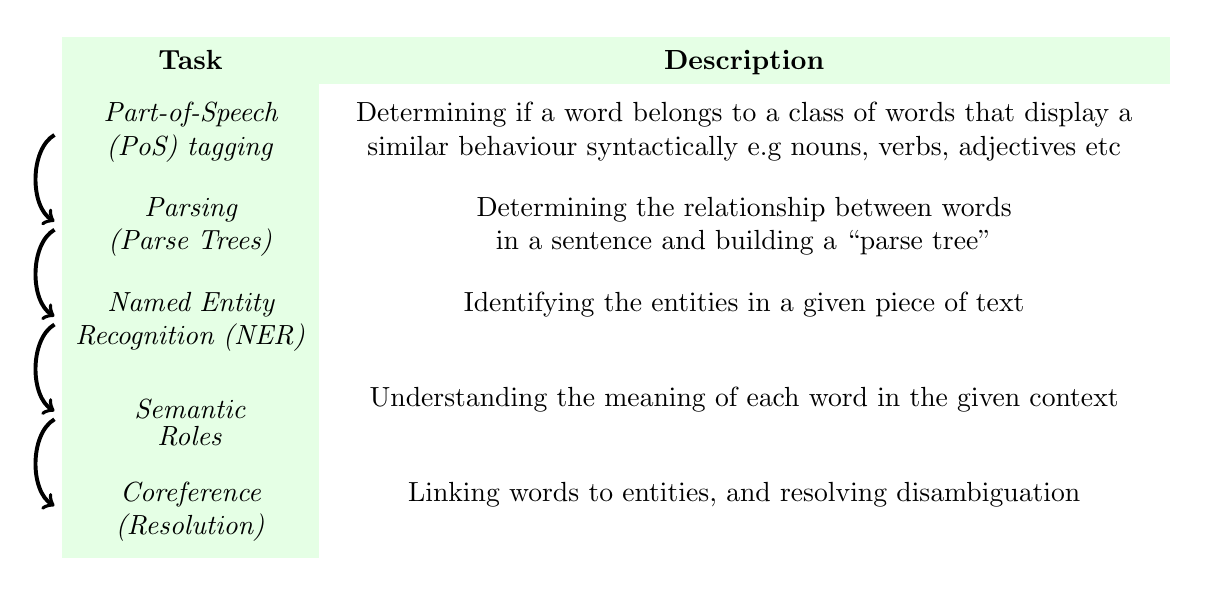
\begin{tikzpicture}[scale=0.8]
		% the matrix entries
		\matrix (mat) [table]
		{
			\textbf{Task} & \textbf{Description} \\
			\textit{Part-of-Speech (PoS) tagging}& Determining if a word belongs to a class of words that display a similar behaviour syntactically e.g nouns, verbs, adjectives etc \\
			\textit{Parsing (Parse Trees)} & Determining the relationship between words in a sentence and building a ``parse tree" \\
			\textit{Named Entity Recognition (NER)} & Identifying the entities in a given piece of text \\
			\raisebox{-5mm}{\shortstack{\textit{Semantic}\\ \textit{Roles}}}  & Understanding the meaning of each word in the given context \\
			\textit{Coreference (Resolution)} & Linking words to entities, and resolving disambiguation \\
		};

		% the arrows
		\begin{scope}[shorten >=3pt,shorten <= 3pt]
		\draw[->, line width=0.5mm]  (mat-2-1.west) to [out=-150,in=150] (mat-3-1.west);
		\draw[->, line width=0.5mm]  (mat-3-1.west) to [out=-150,in=150] (mat-4-1.west);
		\draw[->, line width=0.5mm]  (mat-4-1.west) to [out=-150,in=150] (mat-5-1.west);
		\draw[->, line width=0.5mm]  (mat-5-1.west) to [out=-150,in=150] (mat-6-1.west);
		\end{scope}
	\end{tikzpicture}}
	\captionof{figure}{Potential NLP ``pre-task" pipeline required for a model to solve more complex tasks} \label{fig:intro:nlppipeline}
\end{center}
\section{Thesis Focus} \label{section:intro:projectfocus}
In this section, we briefly describe the key concepts required for the understanding of the aims of the project. All of these sections are fully fleshed out in Chapter \ref{chapter:background}, and include comprehensive relevant literature reviews. For a more detailed description of each section, the reader is referred to Chapter \ref{chapter:background}.

\subsection{Aspect Based Sentiment Analysis} \label{section:intro:absa}
Sentiment Analysis is a subtask of NLP specifically focused on identifying and categorising the emotion or sentiment of a given document (which we use as a general term to refer to any piece of text, including a word, a sentence, a paragraph etc). Typically, the categories are \textit{Positive} and \textit{Negative} in the binary classification case, but this is often extended to include \textit{Neutral}, and sometimes \textit{Conflict} (in the case where both positive and negative sentiment are detected).

Aspect Based Sentiment Analysis (ABSA) granularises this notion further, by performing a sentiment analysis task but for each aspect present in the document (for a fixed list of aspects). An example of this is presented in Figure \ref{fig:intro:absa}.

Target Aspect Based Sentiment Analysis (TABSA) goes one extra step, applying ABSA to a set of target words e.g locations in the text. Thus, ABSA is equivalent to TABSA when there is just one target, namely the object of the sentence.
\begin{center}
	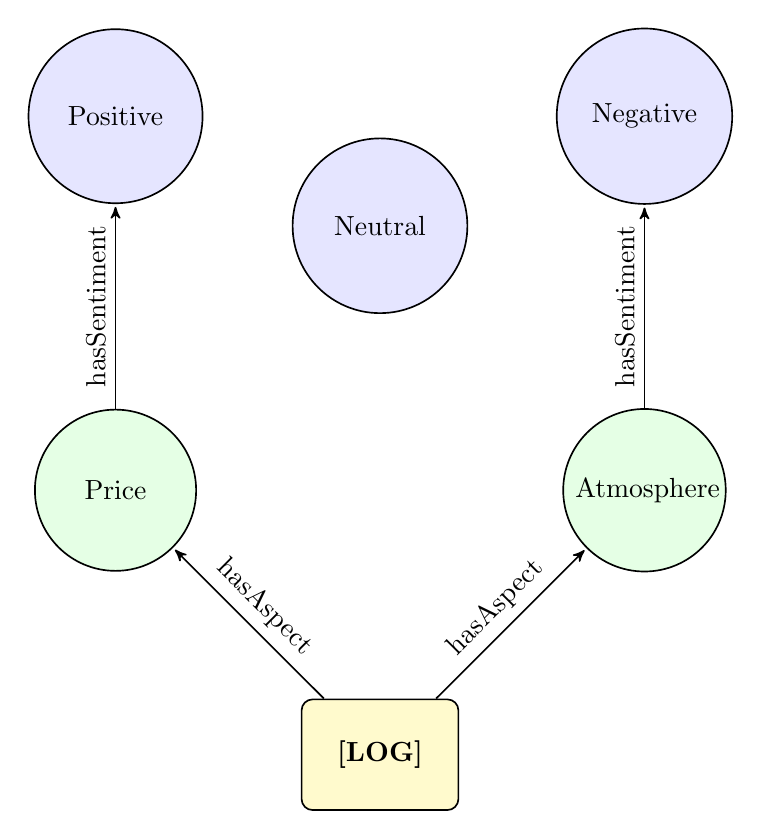
\begin{tikzpicture}[
	->,
	>=stealth',
	shorten >=1pt,
	auto,
	node distance=4.75cm,
	semithick,
	every state/.style={fill=red,draw=none,text=white},
	]
	\node [log, boldtext]        (LOG)                     {[LOG]};
	\node [aspect]         (P) [above left of=LOG]  {Price};
	\node [aspect]         (A) [above right of=LOG]  {Atmosphere};
	\node [sentiment]    (pos) [above of=P] {\Smiley Positive};
	\node [sentiment]    (neut) [above right of=P] {\Neutrey Neutral};
	\node [sentiment]    (neg) [above of=A] {\Sadey Negative};
	%	\node [sentiment]    (chun) [above right of=A] {\Chunny};
	%	\node [sentiment]    (cool) [below of=chun] {\Cooley};
	
	\path[every node/.style={sloped,anchor=south,auto=false}]
	(LOG) edge              node {hasAspect} (P)            
	(LOG) edge              node {hasAspect} (A)
	(P) edge node {hasSentiment} (pos)
	(A) edge node {hasSentiment} (neg);
	\end{tikzpicture}
	\captionof{figure}{Example ABSA Knowledge Graph Construction. \newline Here, \textbf{[LOG]} = ``The restaurant was really cheap, but it didnt have a great vibe". \newline An alternative presentation of the above is that the aspect nodes have sentiment attributes, rather than an additional relation to a seperate node in the graph.} \label{fig:intro:absa}
\end{center}

Above, we have used the terminology ``log" to refer to an input sequence. This aligns with the companies terminology of referring to a specific response to a survey question as a ``log" for that user. See Appendix \ref{appendix:streetbees} for more information.

\subsection{Transfer Learning} \label{section:intro:intrototransfer}
Transfer learning has enabled great progress in the field. The basic premise is that we can pretrain base models on quite general tasks and save the weights, then we can initialise our version of a model using the pretrained, initialised base model and add some additional architecture to \textit{fine tune} the model to our specific task. By fine tuning, we mean randomly initialising some additional architecture that projects onto the task labels for classification tasks or single node for regression tasks and training the model end-to-end on new data. In doing so, we leverage the capabilities of the more general base model by starting in a (locally) optimal region of the model parameter space, enabling effective transfer learning to the specific task at hand. Typically, the task that the model was used for pretraining was in some sense more general than the task required at fine tuning time, meaning the system has formed some internal representation, i.e. ``knowledge", to solve the general task that can then be additionally manipulated to solve the specific task.

Not only do we benefit from the democritisation and distributional nature of research (in that we are able to replicate results without access to the compute or data in which the results were obtained, we can just preload in a set of weights that others have trained) but the notion of transfer learning has foundations in human understanding of our own learning; every time we learn a new task we do not ``start from zero", instead we use our pre-existing knowledge as a basis for improvement. Additionally, the type of scenarios that Transfer Learning benefit from are when large datasets are used for the pretraining, enabling us to fine tune onto tasks with significantly less datapoints.

\subsection{Multitask Learning} \label{section:intro:introtomultitask}
To generalise the notion of Transfer Learning one step further, we may believe that a system capable of performing many tasks simulteneously forms a better representation of each task, since it can learn from related tasks during training and adjust its parameters in a way that \textit{shares knowledge across tasks} in the colearning framework. 

Suppose we were given a set of tasks $\mathcal{T} = \{\tau_1, \dots, \tau_n\}$ that we wanted to learn. Fine tuning/transfer learning would learn each task independently, whereas a clear benefit of multitask learning is that each task is not independent, and colearning encourages a shared knowledge representation. Additionally, this colearning means we can view multitask learning as a form of \textit{inductive transfer}. By introducing an inductive bias, which causes the model to prefer some hypothesis over others, the additional tasks act as a regulariser since the model learns to prefer hypotheses that explain more than one task simultaneously. Another benefit is that suppose we were given a new task $\tau^*$ closely related to some subset of tasks $T \subseteq \mathcal{T}$, then we would typically require less data \cite{Caruana1997} for the new task due to this shared representation of knowledge; from a pedagogical perspective, we often learn tasks first that provide us with the necessary skills to master more complex ones as humans.

\subsection{Meta Learning} \label{section:intro:introtometa}
Faced with a new task $\tau^*$, how do we learn it? With a transfer learning approach, we may require tens of thousands of new examples from which we have to fine tune. With a multitask learning approach, depending on the similarity to the tasks trained on, we may need thousands or tens of thousands of additional datapoints. But what if a system could, given a set of tasks $\mathcal{T} = \{\tau_1, \dots, \tau_n\}$ for pretraining, learn to generalise well to a new task $\tau^*$ with a minimal number of examples. This is the role of meta learning: ``learning to learn".

Multitask pretraining to colearn a shared knowledge representation and testing on task $\tau^*$ is sometimes referred to as \textit{lifelong learning}, and is a form of meta learning, since the meta learning proposition is to learn ``general" properties of a model (e.g weights) that are highly adaptable to new tasks. Recently, focus has shifted onto model agnostic techniques. In the meta learning paradigm, we explicitly train the model to be able to generalise between the tasks in $\mathcal{T}$ so that, at test time, it is able to learn good representations from a test task from a minimal number of examples.

Like multitask learning, meta learning frameworks act as effective regularisers, since they prefer hypotheses that generalise to many tasks.

\section{Project Aims \& Our Contributions} \label{section:intro:projectaims}
The primary aim of this project is to investigate the role of multitask learning applied to Language Models for Aspect Based Sentiment Analysis (ABSA) focusing in particular on:
\begin{itemize}
	\item The role of primary and auxilliary tasks in the training procedure, and identifying suitable secondary subtasks that improve performance in the primary task (ABSA)
	\item How the training procedure influences performance. We do this by defining some novel task sampling schemas (as per Section \ref{section:methodology:taskdistributions}) and investigating their effect on the key metrics.
	\item Investigate the generalisation capability of these systems to previously unseen aspects, including the  introduction a novel application of meta learning to language models for generalising to unseen aspects and comparing this to a lifelong multitask learning approach.
	\item To provide a consistent, open source implementation, of multitask and meta learners applied to language models for the benefit of the research community.
\end{itemize}

The literature on MTL is extensive, but there has never been an investigation on specific hierarchical subtask structures and sampling schemas in direct relation to performance on downstram tasks. In this investigation, we scope a very general problem and compare it against baseline multitask learning techniques. The motivation for our selected sampling schemas compared to the current multitask learning methodologies is outlined in Section \ref{section:background:samplingtasks} and defined thoroughly in Sections \ref{section:methodology:taskstructure} and \ref{section:methodology:taskdistributions}.

In particular, we contribute a detailed investigation of optimal fine tuning procedures in the multitask learning setup to learn complex tasks by relying on supporting subtasks of the complex task, and how best to train an end to end model in terms of sampling from these tasks. We open source our implementation for the benefit of the research community, and this methodology could be applied to any NLP problem and works with a variety of Language Modelling architectures and general downstream classification or regression tasks.

We show that this methodology is valid, in the sense that we outperform all metrics for the (T)ABSA tasks, with our champion model utilising our novel sampling schema. We critically analyse and discuss the results, propose meaningful extensions to this research, and provide useful insights and hypotheses into how the pretraining procedure of large language models can affect the fine tuning procedure. The multitask learning landscape, in particular the interplay between transformer architectures and how they learn meaningfully, is not yet well understood by the research community; we hope that this thesis provides a platform on which future research can be based upon.

\section{Commercial Applications}
Despite being a research project, this thesis topic has strong connections with commercial interests. This code was integrated into the company codebase and productionised for the automatic generation of knowledge graphs.

The framework created for this project (as referenced in Chapter \ref{chapter:methodology} and Appendix \ref{appendix:code}) was extremely flexible, and so could be implemented for a variety of NLP tasks for either research or commericial purposes.

More information on the company and project relevancy can be found in Appendix \ref{appendix:streetbees}, which provides a lot of motivating material for the decisions in the project, and, although these are noted or cited in the thesis document in the relevant locations, the appendix would be welcome introductory background information for the reader.

\section{Public Code Repository}
\label{section:intro:code}
The code accompanying this thesis has been made freely available online via GitHub at:
 \begin{center}
 \href{www.github.com/RyanJenkinson}{\texttt{www.github.com/RyanJenkinson}}.
 \end{center}
In this repository, you can find the library with all of the code, which we have named \texttt{TraMML} - Transformers with Multitask and Meta Learning - as well as this thesis, and all accompanying papers and images. More information regarding specific code implementation and how to run sections of the library can be found in Appendix \ref{appendix:code} or in the \texttt{TraMML} README.


 
\newpage \cleardoublepage

% CHAPTER 2 - BACKGROUND
% ------------------------------------------------
% Nomenclature list - update if needed
\nomenclature[G]{$\mathcal{D}$}{A dataset}
\nomenclature[G]{$\P$}{A probability distribution}
\nomenclature[G]{SOTA}{State of the Art}
\nomenclature[G]{RNN}{Recurrent Neural Network}
\nomenclature[G]{LSTM}{Long Short Term Memory (Network/Architecture)}
\nomenclature[G]{(T)ABSA}{(Target) Aspect Based Sentiment Analysis}
\nomenclature[G]{LM}{Language Model}
\nomenclature[G]{QA}{Question Answering}
\nomenclature[G]{NER}{Named Entity Recognition}
\nomenclature[G]{NLI}{Natural Language Inference - e.g similarity of two sentences or next sentence prediction task}
\nomenclature[G]{NLU}{Natural Language Understanding}
\nomenclature[G]{GLUE}{General Language Understanding Evaluation benchmark - a common set of tasks for which we train, evaluate and analyse NLU systems}
\nomenclature[G]{Support}{We adopt the mathematical definition of support: the number of nonzero points in a domain. In our case, it will refer to the number of instances of examples.}

\nomenclature[L]{ELMo}{Embeddings from Language Models}
\nomenclature[L]{GPT}{Generalised Pre Training}
\nomenclature[L]{RoBERTa}{Robustly optimised BERT approach}

\nomenclature[Z]{$\mathcal{S}$}{Support Set}
\nomenclature[Z]{$\mathcal{Q}$}{Query Set}
% ------------------------------------------------
\chapter{Background} \label{chapter:background}
In this chapter, we give a slightly expanded history of the field of NLP, referencing the evolution of language models building up to the current state of the art (SOTA) models used in this thesis. The critical analyses of the literature review will occur primarily on these works, while the preceding sections act as a prelude. Further, we analyse the field of multitask learning applied to language models, with particular focus on the Sentiment Analysis task, and the more granular Aspect Based Sentiment Analysis (ABSA) task that we will be focusing on in the experimentation element of this thesis.

To be consistent throughout this section, we define a \textit{parameter} of a model as a (set of) number(s) that can be learned directly during the training process - e.g a set of weights or biases - whereas a \textit{hyperparameter} cannot be learned directly during training, but has to be defined \textit{a priori} from the user. These hyperparameters will affect the performance of the model, and typically a (grid or random) search is conducted over some reasonable space in order to optimise what these numbers should be.

\section{The Evolution of Language Modelling}
The goal of this section is to outline various methodologies that lead to us modelling language. Our goal is to find some word representation vector that summarises a word in a given context; i.e. representation learning. We ideally want the word vectors of similar words, such as ``hotel" and ``motel" to be roughly equivalent ($\mathbf{w}_\text{hotel} \approx \mathbf{w}_\text{motel} \Rightarrow \mathbf{w}_\text{hotel} \cdot \mathbf{w}_\text{motel} \approx 1$) since they are used in similar contexts to represent similar things. Learning high quality representations can be challenging, since ideally we should model both the complex characteristics of word use (e.g., syntax and semantics), and how these uses vary across linguistic contexts (i.e. to model polysemy).
\subsection{Problem Setup} \label{section:background:problemsetup}
To formally define the language modelling setup: our goal is to infer a probability distribution $\P$ that predicts the next word given the \textit{context}. For now, the context will refer to all previous words, but we will explore subsets of previous words and surrounding words as contexts in sections \ref{section:background:ngram} and \ref{section:background:bidirectional}. That is, at time $t$ we want to predict word $\mathbf{w}_{t+1}$ given words $\mathbf{w}_{1:t} = \{ \mathbf{w}_1, \dots, \mathbf{w}_t \}$. Each word comes from a vocabulary $V$, so that $\forall i: \mathbf{w}_i \in V = \{\mathbf{w}^{(1)}, \dots, \mathbf{w}^{(|V|)}\} $.

By Bayes Rule, we may write that
\begin{align}
\P(\mathbf{w}_{t+1} | \mathbf{w}_{1:t}) = \frac{\P(\mathbf{w}_{1:(t+1)})}{\P(\mathbf{w}_{1:t})} \approx \frac{\text{count}(\mathbf{w}_{1:(t+1)})}{\text{count}(\mathbf{w}_{1:t})}
\end{align} 
where $\text{count}(\mathbf{w}_{1:i})$ refers to the number of instances of the strings containing $\mathbf{w}_1 \land \dots \land \mathbf{w}_i$ in some (ideally large) corpus of text. Note the commutitivity of the logical \texttt{OR} operation means that sequential structure is not preserved. In addition, this approximation does not scale well with $t$ since the prediction of words given a large context require good counts of very specific long strings in order to get meaningful approximation to the probability, which are unlikely to appear exactly in the corpus. This approach is thus computationally intractable and data inefficient. These can also be referred to as storage and sparsity problems respectively.

\subsection{$n-$gram models} \label{section:background:ngram}
To deal with data inefficiency, we can make a natural simplification that the \textit{context} is not the entire preceding string, but instead the previous $n-1$ words for some chosen (hyperparameter) $n$. The concatenation of $n$ words is called an ``$n-$gram" \cite{Brown}. Clearly, the larger the value of $n$ the more context we have, but the more data inefficient the procedure is as we encounter the same problem as before with the specific $n-$gram being unlikely to appear in our text corpus frequently. The lower the value of $n$ means we are disregarding increasing amounts of contextual information, so this represents a tradeoff for researchers. In practice, often 2-grams (``{{\color{red} bi}grams") and 3-grams (``{{\color{red} tri}grams") are used.

However, we still encounter the sparsity problem. If our $n-$gram in the numerator does not exist in the corpus then our probability distribution would predict that word having probability 0 of occuring, meaning we are biasing our distribution towards the particular corpus(es) used. A partial solution to this is adding some $\varepsilon$ to every word $\mathbf{w} \in V$, called \textit{smoothing}. If the $(n-1)$-gram in the denominator does not exist then our approximate probability distribution is not well defined, but a partial solution is to instead \textit{backoff} to the maximal $(n-k)-$gram that does exist in the corpus. These partial solutions do not fix the overall problem that $n-$gram models tend to exhibit reasonable local structure, but fail to capture long term dependencies and relationships to have any global meaning. We need a smarter model, and one that balances this important interplay between non trivial contextual information and data efficiency.


\subsection{Pretrained Word Embeddings: Humble Beginnings} \label{section:background:wordembeddings}

In the previous sections, we have described the importance of context to language modelling. The first class of methods that ignited research into word embeddings and representations was the Word2Vec models by Google \cite{Mikolov}. They built upon the Skip Gram model \cite{Mikolov2013} to learn distributed vector representations that captured syntactic and semantic word relationships, and proposed extensions that could be applied to the Continuous Bag Of Words (CBOW) model which they also introduced, as seen in Figure \ref{fig:background:SkipGramvsCBOW}. In particular, they introduced some key training techniques such as negative sampling and hierarchical softmax which enabled them to ingest orders of magnitude more training data from which greater amounts of contexts could be seen.

Despite the primitive neural network model, the word vectors are specifically trained to predict the surrounding words in the sentence via backpropagation to maximise the average log probability in a context window of size $c$ and thus the vectors can be seen as representing the distribution of context in which the word appears.

\begin{center}
	\includegraphics[width=.75\textwidth]{CBOWvsSkipGram.png}
	\captionof{figure}{Continuous Bag Of Word (CBOW) models vs Skip Gram Models \newline Skip Gram models predict a words context given the word itself, whereas CBOW models predict a word given its context.}
	\label{fig:background:SkipGramvsCBOW}
\end{center}

GloVe Vectors \cite{Pennington} take a different approach, and propose a weighted least squares model that looks to factorise the (log) word co-occurance matrix. They show that this approach can be formalised mathematically in the setting of an extension proposed by Mikolov \cite{Mikolov}, and do additional training tricks such as filtering the data to reduce the weighting factor for more frequent words during training (since these words appear in many contexts, and thus dont carry as much information).

Since the methods they proposed could ingest larger still amounts of context by leveraging age-old scalable mathematical optimsiation routines \cite{Pennington}, their results proved state of the art, as well as the fact that they were much more sample efficient, with accuracies around 4\% higher than the CBOW or Skip-Gram methods given the same compute time.

The important factor about these methods, is that the word embeddings captured contextual structure. We can look at a lower dimensional representation of the embedding space using dimensionality reduction techniques, for example tSNE \cite{VanDerMaaten2008}, which uses a stochastic neighbour embedding that aims to approximate the high dimensional structure in the form of a similarity matrix of conditional probabilities between datapoints with a lower dimensional onevoptimised by minimising the Kullback-Leibler Divergence \cite{Kullback1951}, to find that \textit{similar words occupy similar regions of the embedding space}. This indicates that the embedding space learned captures contextual information, since words close in the embedding space are ``associative neighbours" \footnote{in the linguistic sense, an associative neighbour $y$ of a word $x$ is a word such that when $x$ is replaced by $y$ in a given context, the sentence still makes sense.} - this is demonstrated in Figure \ref{fig:background:wordembeddings}. Interestingly, we can define an algebra in this space, in the sense that the relationship between clusters of words are represented by similar vectors (e.g tenses, but also more complex world information such as country-capital).

\begin{center}
	\includegraphics[width=.75\textwidth]{wordembeddings.png} \\
	\includegraphics[width=.75\textwidth]{wordalgebra.png}
	\captionof{figure}{The reduced dimensionality word embedding space found using \texttt{word2vec} \cite{Mikolov} and the algebraic relationship between clusters of words in this space}
	\label{fig:background:wordembeddings}
\end{center}

\subsection{The Rise of Deep Learning: Using Sequentiality for Context} \label{section:background:bidirectional}
Deep learning successes tend to come in the large data regime. The distributional semantics hypothesis proposed by Saussure (as discussed in Section \ref{section:intro:history}) can apply directly here, since we simply need to ingest lots of data about how words are used and in which contexts and this is, in a sense, all we need to know about the word (e.g we don't need to form any external world view or model, a word is entirely defined by the contexts it is used in). The previous section highlights that word vectors are effective in capturing contextual information, and in this section we explore deeply uni/bi-directional models.

The disadvantage of the methods previously discussed is that it might be good to have a good representation for each word, but how do we combine them? As a baseline we could, once we have a good word representation, just ``average the words (embeddings)" to get a sentence embedding. This has its drawbacks, however, in that we lose the word order and sequentiality structure. We focus, now, on networks that take into account the sequential structure that gained traction in the field, that build upon these simply averaging/concatenation models of word embeddings to.

\subsubsection{Recurrent Neural Networks}
Recurrent Neural Networks \cite{Elman1990} are an ideal choice to deal with dynamic length input sequences that are prevalent in all NLP tasks. They are defined by two simple equations: RNNs store a hidden state representation at every timestep (which here corresponds to a word/token in the sentence) and they use this hidden state $\mathbf{h}_t$ to: (a) update its hidden state representation at the next time step whilst including information about the current time steps (i.e word) input and (b) make a prediction based on this hidden state at each time step. They are optimised using backpropagation through time \cite{Werbos}. For input $\mathbf{x}_t$ and hidden state $\mathbf{h}_t$ at time $t$, weight matrices $W_i$ and biases $\mathbf{b}_{\{h,o\}}$ we can get the prediction at time $t+1$, $\hat{\mathbf{y}}_{t+1}$ with the update rules:
\begin{align}
\mathbf{h}_{t+1} = \sigma \left(W_1 \mathbf{x}_{t+1} + W_2 \mathbf{h}_t + \mathbf{b}_h \right) \tag{a} \\
\hat{\mathbf{y}}_{t+1} = \text{softmax}\left(W_3 \mathbf{h}_{t+1} + \mathbf{b}_o \right) \tag{b}
\end{align}
 However, they suffered from vanishing and exploding gradient problems \cite{Pascanu}, where the backpropagation of the gradient through the network would prove in practice unstable, since the product of matrices unrolling through time can shrink to 0 or grow to infinity (along some direction $\mathbf{v}$) in value.

The proposed solution to this was introduced was a Long Short Term Memory (LSTM) Network \cite{Hochreiter1997}, which is similar to a RNN except the inclusion of gates which allow information to propagate through a ``cell". It keeps a hidden cell state of accumulated ``memory" and decides how much of the information from the next word in the sequence should be incorporated into its hidden state.

\begin{center}
	\includegraphics[width=.75\textwidth]{lstm.png}
	\captionof{figure}{One LSTM cell with corresponding equations, image taken from \cite{Varsamopoulos2018}. There is one cell for each word in the input sentence. We input embedding $x_t$, and propagate forward the hidden state $h_t$ and the cell state $C_t$. $\{i_t, f_t, o_t\}$ are the \{input, forget, output\} gates, $W^{\{i,f,o\}}$ and $U^{\{i,f,o\}}$ are learnable weight matrices.}
	\label{fig:background:lstm}
\end{center}

Following from this, Graves et al. showcased the power of Deep \textit{Bidirectional} LSTM (DBLSTM) networks for speech recognition temporal classification task \cite{Graves2013}. This small yet powerful modification allows the model to account for both sequential directions of context, and gives a much richer word representation since we can account for downstream words/tokens as opposed to just words/tokens seen prior to the current word at timestep $t$. It achieves this as per Figure \ref{fig:background:bidirectionallstm}, by implementing two LSTM models in parallel, one propagating forward through the input tokens and the other propagating backward through the input tokens, and concatenating together the hidden states of each model into a hidden state for the entire architecture. Then, inference is performed as above.

\begin{center}
	\includegraphics[width=.75\textwidth]{bidirectionallstm.png}
	\captionof{figure}{Bidirectional LSTM architecture as defined in \cite{Graves2013}}
	\label{fig:background:bidirectionallstm}
\end{center}

\subsubsection{ELMo \& GPT}
There have been many works to get rich context embeddings, but one of the most successful was ELMo \cite{Peters2018a} (\underline{E}mbeddings from \underline{L}anguage \underline{Mo}dels). Building upon the work of context dependent representations with bidirectional LSTM networks, ELMo embeddings utilise the DBLSTM architecture, but add regularisation and task specific weightings of all the hidden bidirectional layer represenations. Thus, unlike traditional word embeddings in Section \ref{section:background:wordembeddings}, the word representations are functions of the entire input sequence.

ELMo \cite{Peters2018a} proposes to extract context-sensitive features from a language model. OpenAI's GPT (Generalised Pre Training) Language Model \cite{RadfordGPT}, however, enhances the context-sensitive embedding by adjusting the Transformer architecture \cite{Vaswani}. Since the transformer architecture is utilised in the current state of the art models, treatment and analysis of this architecture is deferred to section \ref{section:background:LMs}. While the GPT Model did not outperform SOTA Sentiment Analysis, it achieved SOTA on 9 out of 12 NLP tasks, and provided an important stepping stone to the state of the art language models, showcasing the power of the TransformerXL \cite{Dai2019} architecture, which actually enables learning dependency beyond a fixed context width unlike the other recurrent models through having recurrent mechanisms inside the architecture focusing on certain ``segments". However, this is still a ``standard" language modelling setup in the sense that it is a unidirectional model. The importance of this paper was to set up the following paradigm: \textit{generative pre-training} of a language model on a diverse corpus of unlabeled text, followed by \textit{discriminative fine-tuning} on each specific downstream task. This is the paradigm we use throughout this thesis, and this paper first demonstrated its efficacy on a range of downstream tasks including absolute improvements of 8.9\% on commonsense reasoning tasks, 5.7\% on question answering tasks, and 1.5\% on textual entailment tasks.

\section{Current SOTA Language Modelling: Transformers} \label{section:background:LMs}
The previous section provides a basis of understanding on which the current state of the art models are built upon. We outlined important ideas of bidirectional context embeddings, and explore further in this section how state of the art language models have been built. These are the models that were implemented for our experiments (outlined in Chapter \ref{chapter:experiments}), and what we built additional functionality on top of.

Following the successes of inductive transfer learning applied to Computer Vision \cite{He2015, Huang2016}, where large convolutional and residual architectures were pretrained on large common image datasets such as ImageNet \cite{ImageNet} and COCO \cite{COCO}, focus was redirected onto training large pretrained models that would act as a Language Model. Up until this point, Deep Learning had showed promise in achieving state of the art on many different NLP tasks, but there was rarely a consistent model architecture (since researchers often hand crafted task specific architectures in order to achieve SOTA performance), and these models were often trained from scratch which required large datasets and days to converge. In 2018, researchers proposed Universal Language Model Fine-tuning (ULMFiT) \cite{Howard2018}, an effective transfer learning method that could be applied to any task in NLP, and introduced key techniques for fine-tuning a language model.

Their aim, as is common to all subsequent language model variants, was to define a model that was expressive enough to, in a sense, ``capture language" via a (set of) suitable pretraining task(s). Such a model could ingest large quantities of unlabelled text data, and learn ``good" (contextualised) word embeddings. Then, the classifier could be fine tuned (via subsequent linear layers) to capture the idiosyncracies of the downstream target task (especially if the target task was different from the pretraining task). This would require additional data, but the premise of transfer learning is that it requires orders of magnitude less training data than training a model from scratch, since it can leverage pre-existing knowledge in the form of the pretrained word embeddings \cite{RuderThesis}.
\subsection{Transformer Architecture}
While prior models relied on convolutional or recurrent architectures, in 2017 researchers proposed a novel architecture: the Transformer \cite{Vaswani}, based solely on \textit{attention mechanisms}, dispensing with recurrence and convolutions frameworks entirely. They found in experiments on two machine translation tasks that these models were superior in quality but, more importantly, they demonstrated the models ability to be more parallelizable and requiring significantly less time to train than previous models. This would allow for the ingestion of more data from which to learn in a given time frame and potentially yield much more powerful models.

\subsubsection{Attention: An Introduction}
Self-attention, sometimes called intra-attention, is an attention mechanism relating different positions of a single sequence in order to compute a representation of the sequence. Self-attention had been used successfully in a variety of tasks including reading comprehension, abstractive summarization, textual entailment and learning task-independent sentence representations prior to the Transformer network \cite{Cheng2016, Parikh, Paulus2017, Lin2017}, but the Transformer network was the first end-to-end transduction model relying entirely on self-attention to compute representations of its input and output without using any recurrent or convolution elements.

The reader is referred to the diagram in Figure \ref{fig:background:transformer} taken from the original paper, but we first describe all the components of the diagram in detail.

\subsubsection{Encoder and Decoder Architecture}
\textbf{Encoder:} The encoder is composed of a stack of $N$ identical layers, with two sub-layers: the first is a multi-head self-attention mechanism, and the second is a fully connected feed forward (linear) layer. The authors utilise a residual connection \cite{He2015} around each of the sublayers, as well as employing layer normalization \cite{Ba2016}. All sub-layers in the model, as well as the embedding layers, produce outputs of dimension $d_\text{model}$.

\noindent \textbf{Decoder:} The decoder is also composed of a stack of $N$ identical layers: as well as the two sub-layers in each encoder layer, the decoder inserts an additional third sub-layer, which performs multi-head attention over the output of the encoder stack. As before, the authors use residual connections around each of the sub-layers, followed by layer normalization. They also modify the self-attention sublayer in the decoder stack to prevent positions from attending to subsequent positions. They refer to this as \textit{masked self attention} and this, combined with fact that the output embeddings are offset by one position, ensures that the predictions for position $i$ can depend only on the known outputs at positions less than $i$ (i.e it cannot see itself or into the future).

\subsubsection{Attention: The Mathematical Formalism}
An attention function can be described as mapping a \textit{query} and a set of \textit{key-value} pairs to an \textit{output}, where the query, keys, values, and output are all vectors of dimensionalities $d_k, d_k, d_v, d_\text{model}$, respectively. The output is computed as a weighted sum of the values, where the weight assigned to each value is computed by a compatibility function of the query with the corresponding key.

The authors compute the attention function, which they called ``Scaled Dot Product Attention" on a set of queries simultaneously, packed together into a matrix $Q$. The keys and values are also packed together into matrices $K$ and $V$, respectively. Then, the matrix of outputs is computed as:
\begin{align*}
\text{Attention}(Q, K, V) = \text{softmax}\left( \frac{QK^T}{\sqrt{d_k}} \right) V
\end{align*}
where the inverse of the square root of $d_k$, the dimensionality of the keys (and also queries), provides a scaling factor since the dot product between the keys and the queries can get large. The first term provides ``attention weights" which determine the linear combination of the values $V$. In essence, we see how similar the query is to each of the keys, then take a corresponding simililarity weighted linear combination of the values corresponding to those keys.

Multi-headed attention allows the model to jointly attend to information from different representation subspaces at different positions, with the intuition that, as well as providing a form of regularisation to the model, the model can attend to ``different types of things in each head" since it forms a specific representation in each one. Formally, we can write:
\begin{align*}
\text{MultiHead}(Q,K, V) &= \text{Concat}(\text{head}_1, \dots, \text{head}_h) W^O \\
\text{where head}_i &= \text{Attention}(Q W_i^Q ,K W_i^K , V W_i^V )
\end{align*}

where the projections into each head subspace are parameter matrices:
\begin{align*}
W_i^Q \in \mathbb{R}^{d_\text{model} \times d_k} , W_i^K \in \mathbb{R}^{d_\text{model} \times d_k} , W_i^V \in \mathbb{R}^{d_\text{model} \times d_v} \text{ and } W^O \in \mathbb{R}^{h\cdot d_v \times d_\text{model}}
\end{align*}

\begin{center}
	\includegraphics[width=\textwidth]{TransformerArchitecture.png}
	\captionof{figure}{The Architecture of the Transformer Model \cite{Vaswani}}
	\label{fig:background:transformer}
\end{center}

\subsubsection{Benefits of Self Attention}
There are many benefits of an end-to-end attention model over traditional recurrent or convolutional models, in particular the computational complexity per layer (compared in detail in Table 1 in \cite{Vaswani}), the amount of parallelisation computations (due to the lack of sequentiality needed - a major limitation identified in Section \ref{section:background:bidirectional})), and the path lengths the information has to travel in both forward backpropagation passes (of the gradients of the loss through the network) which can destabilise the learning procedure.

The authors note of an additional benefit: interpretability of models. They inspect attention distributions from their models and present and discuss examples in the appendix. They find that individual attention heads clearly learn to perform different tasks, many appear to exhibit behavior related to the syntactic and semantic structure of the sentences, although recent papers \cite{Jain} have disputed this claim having found that after running extensive experiments on a variety of NLP tasks, the attention distributions are uncorrelated with gradient-based measures of feature importance, and one can identify very different attention distributions that nonetheless yield equivalent predictions. Research in this area is ongoing, and outside the scope of this thesis.

\subsection{BERT} \label{section:background:bert}
\begin{center}
	\includegraphics[width=\textwidth]{BERTvsELMovsGPT.pdf}
	\captionof{figure}{BERT vs OpenAI GPT vs ELMo}
\end{center}
In 2018, a powerful deep learning model was introduced to the NLP community by researchers at Google. BERT (\underline{B}idirectional \underline{E}ncoder \underline{R}epresentations from \underline{T}ransformers) \cite{Devlin2018} was an extremely powerful model, but very different from others around at the time, since it was designed to pretrain deep bidirectional representations by jointly conditioning on both left and right context in all layers. As a result, the learned language manifold was so powerful that fine tuning only required one additional linear layer to be learned for the downstream tasks. Clearly, this was much more sample efficient than previous methods, and it obtained new SOTA performance on 11 NLP tasks, pushing the GLUE (General Language Understanding Evaluation) benchmark \cite{Wang2018} up by a 7.6\% absolute improvement to 80.4\% at the time of paper release. This task is a collection of subtasks that benchmark NLU models on a range of downstream tasks, including Question Answering (QA), Natural Language Inference (NLI) and Sentiment Analysis tasks.

Intuitively, it seems obvious that a deep bidirectional encoding would perform strictly better than a left-to-right or right-to-left model, as well as the concatenation of such models, but traditional conditional language models have not been trained in this way since bidirectional conditioning would allow each word to indirectly ``see itself" in a multi-layered context. The authors avoid this by a novel innovation inspired by the Cloze \cite{Taylor1953} task: the Masked Language Model (MLM). The masked language model randomly masks some of the tokens from the input, and the objective is to predict the original vocabulary id of the masked word based only on its context. Unlike traditional unidirectional language model pre-training, the MLM objective allows the representation to fuse the left and right context, which allowed them to pre-train a deep bidirectional Transformer.

\subsubsection{Masked Language Modelling - Cloze Task}
In the MLM, the idea is to mask out $k$\% of the tokens (the BERT authors consistently use $k=15$). They augment the token set with a special \texttt{[MASK]} token and while this allows them to achieve bidirectionality (since the model does not know which word will get masked, it is forced to keep a contextual word representation of all words in the sentence) it does come with its downsides: firstly there is a misalignment between the pretraining procedure and test-time procedure, since the \texttt{[MASK]} token is never seen at test time. To mitigate this, they do not always replace ``masked" words with the actual \texttt{[MASK]} token (instead of always replacing the chosen words with \texttt{[MASK]}, 80\% of the time they replace it with \texttt{[MASK]}, 10\% of the time they replace it with a random word and 10\% of the time they leave the word unchanged in order to bias the representation towards the actual observed word), and secondly, since only $k$\% of tokens (the \texttt{[MASK]} tokens) are predicted in each batch, rather than every token for traditional language models, we expect less sample efficiency and more pre-training steps may be required for the model to converge. This indeed turns out to be the case, although recent papers \cite{Liu2019} have shown that with simple modifications to the BERT pretraining procedure\footnote{(1) training the model longer, with bigger batches, over more data; (2) removing the next sentence prediction objective; (3) training on longer sequences; and (4) dynamically changing the masking pattern applied to the training data.} and a careful analysis of hyperparameters allow the BERT model to perform significantly better, concluding that the original authors significantly undertrained the model and that such a pretraining procedure can match or exceed all post-BERT models in terms of performance on downstream tasks. They called this \underline{R}obustly \underline{o}ptimised \underline{BERT} \underline{a}pproach: RoBERTa.

\subsubsection{WordPiece Tokenisation}
Another important undermentioned contribution from the paper was the use of WordPiece tokenisation \cite{Wu2016} with a 30,000 token vocabulary, denoting split word pieces with the prefix \texttt{\#\#}. This allows for common subparts of words to have their own embeddings and thus have a larger general vocabulary since words can be decomposed into their respective word pieces (or \texttt{[UNK]} if unknown). For example: \texttt{doing} $\rightarrow$ \texttt{do \#\#ing}, since the suffix ``ing" is common among many words, and so it has its own embedding. This is particularly useful when subparts of words have their own meanings, e.g in German.

One criticism of the BERT procedure worth noting at this point is that researchers implemented the masking procedure so it applies to \textit{tokens} and not \textit{words}. This was recently corrected, so that when masking a word, if it were split into several tokens then all of those tokens would be masked out simultaneously\footnote{See the online code implementation update at \href{https://github.com/google-research/bert}{\texttt{https://github.com/google-research/bert}}}, but the generic BERT-Base and Large models in all languages had this token masking, meaning that words could effectively ``see themselves" in terms of embeddings (e.g if a word was split into two, it might be that only one of those tokens was masked out, so in predicting that mask it could use information from the other wordpiece as part of the same word). This isnt exactly the correct data corruption model in terms of predicting whole words, and so the training procedure isnt as effective as it should be.

\subsubsection{Next Sentence Prediction Pretraining task}
Importantly for this thesis, as we will explore in Section \ref{section:experiments:nlipretrainingimportance}, the BERT pretraining procedure is augmented with a ``next sentence prediction" task, with two labels (binary): \texttt{isNextSentence} $\in \{0,1\}$. Many important downstream tasks such as Question Answering (QA) and Natural Language Inference (NLI) are based on understanding the relationship between two text sentences, which is not directly captured by language modeling. The authors define segment embeddings to label sentence \texttt{A} (the first sentence) and sentence \texttt{B} (the second sentence) so that during pretraining they choose sentences \texttt{A} and \texttt{B} so that 50\% of the time \texttt{B} is the actual next sentence that follows \texttt{A}, and 50\% of the time it is a random sentence from the corpus, and backpropagate the loss from this additional task through the model.

\subsubsection{Token Structure}
The token sequence is prepended with a special \texttt{[CLS]} token, which represents the hidden embedding used for classification (with the hopes that the learned contextual representation of this token will absorb contextual information from the sentence(s) fed in). A special separator token \texttt{[SEP]} is appended to each sentence (depending on if there is one or two fed into the model) and the sentence is padded up to the maximum sequence length\footnote{512 for the initial BERT models} and then an embedding is learned for each token. Predictions are made on downstream tasks as in Figure \ref{fig:background:berttokenprediction}.

\begin{center}
	\includegraphics[width=.9\textwidth]{BERTTokenPrediction.png}
	\captionof{figure}{BERT Token Prediction}
	\label{fig:background:berttokenprediction}
\end{center}

Additionally, the model learns specific segment embeddings, which better enables it to separate out and distringuish the two sentences (if both are fed) as input. Finally, since the locations of the tokens in the input sentence matters, and gives termporal information to the model. This is because Transformers do not encode the sequential nature of their inputs \cite{Vaswani} and so this is added as an additional embedding. The three embeddings are summed together, as per the diagram in Figure \ref{fig:background:bertembeddings}.

\begin{center}
	\includegraphics[width=\textwidth]{BERTEmbeddings.pdf}
	\captionof{figure}{BERT Embeddings. In addition to the learned token embeddings, there are segment embeddings (as to whether or not we are in the first sentence or second sentence) and positional embeddings \cite{Vaswani} that help indicate the relative positioning of tokens in the sentence.}
	\label{fig:background:bertembeddings}
\end{center}

\subsubsection{Ablation Study}
The original BERT ablation study looked at 3 model variants:
\begin{enumerate}
	\itemsep0em 
	\item A model with a MLM but without the Next Sentence Prediction (NSP) task
	\item A unidirectional left-to-right LM without NSP
	\item Model above + biLSTM (randomly initialised) thereby ``strengthening" the above model
\end{enumerate}
They showed (Table 5 in \cite{Devlin2018}) that including the NSP task improved the model across all tasks, with major improvements, as expected, on the QNLI task (Question Natural Language Inference, a subtask of the Stanford Question Answering dataset). Additionally, they found that the bidirectional model outperformed the unidirectional one.

While subsequent studies (RoBERTa \cite{Liu2019}, XLNet \cite{Yang2019}, ``Fair XLNet" \cite{XLNetTeam2019}) have agreed with the latter claim, they both disagree with the former, instead finding that next sentence prediction as an auxilliary pretraining task \textit{harms model performance}, including on Question Answering and NLI datasets such as SQuAD and MNLI as well as Sentiment tasks (SST-2 - See Section \ref{section:background:sst2}). Additionally, in the ``Fair XLNet" study, they report different best performing BERT models, claiming that the BERT model trained without the NSP task does perform better than the one trained jointly with it \cite{XLNetTeam2019}. This juxtaposition is explored and tested further in our experimental setup in Section \ref{section:experiments:nlipretrainingimportance}.

\subsubsection{Recreating the NLP Pipeline}
In Section \ref{section:intro:history}, we introduced the NLP pipeline, a notional idea that smaller subtasks are required as ``building blocks" of language understanding, and that any model capable of understanding such downstream language tasks must, in some sense, be able to reconstruct this pipeline. Recently, an interesting paper \cite{Tenney2019} conducted by researchers at Google remarked that certain liguistic information was captured in various layers of the network. By introducing a technique they call ``edge probling" they conclude that different layers of the BERT network can resolve syntactic and semantic structure within a sentence, indicating that the model has some explainability and parallels to human cognition in terms of how it understands language. This makes BERT a prime Language Model for our downstream tasks, since it gives us confidence that this model is able to utilise these subtasks for more important tasks of interest.

\begin{center}
	\includegraphics[width=\textwidth]{BERTNLPPipeline.jpg}
	\captionof{figure}{BERT correcting its predictions along the model depth layers, taken from \cite{Tenney2019}}
\end{center}

\subsection{XLNet} \label{section:background:xlnet}
\subsubsection{Autoregressive vs Autoencoding Language Modelling: BERT vs XLNet}
The formulation described in Section \ref{section:background:problemsetup} is referred to as the autoregressive (AR) model. It intends to factorise the likelihood of an input sequence $\mathbf{x} = (w_1, w_2, \dots, w_n)$ into a forward product, or a backward product:
\begin{align*}
\text{Forward Product:} \ & \ \P(\mathbf{x}) = \prod \limits_{t=1}^{T} \P(w_t | \{w_{>t}\}) \\
\text{Backward Product:} \ & \ \P(\mathbf{x}) = \prod \limits_{t=1}^{T} \P(w_t | \{w_{<t}\}) 
\end{align*}
A parametric model (e.g. a neural network) is trained to model each conditional distribution. Since an AR language model is only trained to encode a unidirectional context (either forward or backward), it is not effective at modeling deep bidirectional contexts which we've seen is important for downstream tasks.

As explained in Section \ref{section:background:bert}, BERT gets around this problem by instead using an autoencoding (AE) model; the pretraining does not perform explicit density estimation but instead aims to reconstruct the original data from corrupted input (the \texttt{[MASK]} tokens in BERT). As we've discussed, these artificial \texttt{[MASK]} symbols used by BERT during pretraining are absent from real data at finetuning time, resulting in a pretrain-finetune discrepancy. Furthermore, since the predicted tokens are masked in the input, BERT is not able to model the joint probability using the product rule as in AR language modeling. In other words, BERT assumes the predicted tokens are independent of each other given the unmasked tokens, which is oversimplified as high-order, long-range dependency is prevalent in natural language \cite{Dai2019}.

\subsubsection{Permutation Language Modelling - An alternative pretraining objective}
As a consequence, the authors of XLNet propose a generalized autoregressive method that leverages the best of both AR and AE language modeling and while avoiding their limitations, namely:
\begin{itemize}
	\item Introducing a novel pretraining procedure: fixing either a forward or backward product factorisation but maximise the expected likelihood over \textit{all possible permutations of the factorisation order}. This permutation procedure enables the model to capture bidirectional context since left and right tokens could feasibly appear ``ahead" of the current tokens in the unidirectional model.
	\item As a generalized AR language model, XLNet does not suffer from the pretrain-finetune discrepancy that BERT is subject to. Meanwhile, the autoregressive objective also provides a natural way to use the product rule for factorizing the joint probability of the predicted tokens, eliminating the independence assumption made in BERT.
\end{itemize}
This latter point is important, and the example given in the paper demonstrates the key difference: consider a concrete example [New, York, is, a, city]. Suppose both BERT and XLNet select the two tokens [New, York] as the prediction targets and maximize $\log p(\text{New York} | \text{is a city})$. Also suppose that XLNet samples the factorization order [is, a, city, New, York]. In this case, BERT and XLNet respectively reduce to the following objectives:
\begin{align*}
\mathcal{J}_{\text{BERT}} = \log p(\text{New} | \text{is a city}) + \log p(\text{York} | \text{is a city}) \\
\mathcal{J}_{\text{XLNet}} = \log p(\text{New} | \text{is a city}) + \log p(\text{York} | \text{ {\color{blue} New}, is a city})
\end{align*}
Thus, XLNet is able to capture the dependency between the pair (New, York) which is omitted by BERT, and this leads to a much more effective training signal since XLNet will always be able to capture denser dependency links given this permutation structure and objective.

\subsubsection{Ablation Study}
To investigate the efficacy of the alternative permutation language modelling pretraining objective, as well as design choices such as (importantly to this thesis) the inclusion of the next sentence prediction task, the authors include a comparison of 6 XLNet model variants compared to the original BERT-Base implementation \cite{Devlin2018}. For fair comparison, all models are based on a 12-layer architecture with the same model hyper-parameters as BERT-Base and are trained on only Wikipedia and the BooksCorpus data. They find that the various base models of XLNet outperform BERT on a wide range of tasks, 20 NLP tasks in total. \textbf{maybe include some more numbers and metrics}

Interestingly, the authors note that the inclusion of the next sentence prediction task discussed by the BERT authors harms the model performance across a wide variety of datasets including SST-2 and, more interestingly, MNLI and SQuAD (since, as discussed in Section \ref{section:background:bert}, intuitively we would expect NLI/QA downstream tasks to benefit from NLI pretraining task knowledge), but not RACE (a more challenging reading comprehension task than SQuAD). This feels like an important juxtaposition that is not thoroughly investigated by the authors, and a more rigorous analysis of the next sentence prediction task on NLI and QA downstream tasks should be included, to understand better whether this multitask pretraining objective is a useful feature. Nonetheless, the authors conclude that it is unhelpful, and so omit this auxilliary pretraining objective when training the larger XLNet-Large model. The released set of weights for XLNet-Base do not include this next sentence prediction task, and this is important for a key research question that we investigate in Section \ref{section:experiments:nlipretrainingimportance}.

As discussed in Section \ref{section:background:bert}, a recent paper \cite{Liu2019} showcased that improvements and a more thorough hyperparameter study can lead to BERT, and thus the AE modelling approach, equal or surpass that of XLNet in terms of performance on downstream tasks almost unilaterally.

\subsubsection{Comparisons with BERT}
Upon release of the XLNet paper, the scientific community felt it was unfair to draw direct comparisons between BERT and XLNet, since XLNet used around 10 times more data compared to BERT. Subsequently, the authors followed up the paper with an addendum in the form of a blog post \cite{XLNetTeam2019} where they ensured that almost every possible hyperparameter was the same for both BERT and XLNet as well as pretraining on exactly the same data. 

The study trains 3 separate BERT models, the first being the original one released by the authors, the second being the original model with whole word masking as released by the authors and the third being BERT without the Next Sentence Prediction (NSP) pretraining task since they found the NSP task to harm performance. Despite the Ablation Study in BERT explicitly finding that this task helped in BERT-Base, the XLNet authors report that when training BERT-Large, the best of three variants was often model 2 (10/13 metrics), but occasionally model 3 (3/13 metrics), and never model 1 (0/13 metrics).

They report that even taking the best of these three models, XLNet strictly outperforms BERT across the board on 13 metrics across 11 tasks, albeit by smaller margins than before when it used 10x more data, thus concluding that this model is strictly better than BERT. Recently, however, RoBERTa \cite{Liu2019} ensured the BERT pretraining procedure was much more robust, leading to equal or better performance in XLNet. These transformer architectures, the interplay between pretraining procedures and downstream fine tuning performance and the relationship between larger and smaller models is not yet well understood by the academic community.

\subsection{Casing in Language Models} \label{section:background:casing}
Language models use a tokenizer to preprocess the input words. Both XLNet and BERT use a type of sentence piece tokenisation methodology to split up words into subpieces that are fed in as tokens. There are typically two settings for this, either capitalisation is preserved (\texttt{cased}) or all the inputs are preprocessed into lower case (\texttt{uncased}).

The BERT models release both \texttt{cased} and \texttt{uncased} versions, with vocabulary sizes of 28,996 and 30522 respectively. The lesser vocabulary size in the cased version, as well as the fact that there are often two sets of the same wordpiece token (one with capitalisation, one without) means that the BERT-\texttt{cased} version tends to have worse learned word representations compared to BERT-\texttt{uncased}. The XLNet models are \texttt{cased} by default. Furthermore, both XLNet and BERT have ``base" versions with fewer parameters, and ``large" versions with more parameters.

Typically, researchers use \texttt{bert-base-uncased} in their research since it has fewer parameters and better learned word representations. Since the XLNet models are so new, not much research has been conducted using them at the time of writing this thesis.

\section{Sentiment Analysis}
Sentiment Analysis is an important downstream task for language modelling. Indeed, one such benchmark dataset for the evaluation of language models is GLUE \cite{Wang2018}, a collection of 9 natural language understanding tasks,  of which the SST-2 (see Section \ref{section:background:sst2})  dataset is a subtask. Often, we fine tune these aforementioned language models on these tasks and, after a hyperparameter search or combination with ensemble models (using multitask learning, as discussed in \ref{section:background:multitasklearningforLMs}), achieve higher metrics scores than custom built models trained from scratch.

A more profound demonstration of sentiment's latent utility in text understanding was a paper \cite{Radford2017} which found that when given sufficient amounts of capacity, training data, and compute time, the representations learned by generative models training to generate customer reviews included disentangled features corresponding to high-level concepts, specifically they found a single unit which performs sentiment analysis. They termed this the ``Unsupervised Sentiment Neuron". These representations, learned in an unsupervised manner, achieved state of the art on the binary subset of the Stanford Sentiment Treebank (SST-2, as discussed in Section \ref{section:background:sst2}).

Sentiment Analysis has often been viewed as a human aspect due to the complex contextual and semantic factors involved, but this makes it an interesting and difficult problem for NLP models that are interesting in the academic sense, but also applicable in the commercial setting (cf. Appendix \ref{appendix:streetbees}). In this section, we outline the key Sentiment Analysis tasks that we will focus on in this thesis.

\subsection{SST-2} \label{section:background:sst2}
The Stanford Sentiment Treebank (SST) is a binary (2 class) or fine grained (5 class) single-sentence classification task consisting of sentences extracted from movie reviews with human annotations of their sentiment \cite{Socher}. It is a popular task on which to test Sentiment Analysis performance, and is included as part of the GLUE tasks.

The aforementioned ``Unsupervised Sentiment Neuron" LSTM model achieved an accuracy of 91.8 on the Binary SST-2 dataset. With the advent of fine tuning language models, we achieved much better accuracy scores than these custom built models. BERT achieved a score of 94.9, an impressive absolute increase of 3\%, further justifying the capabilities of a pretrained language model, and XLNet achieved the (current SOTA) accuracy of 96.8\%, utilising an ensemble model of the larger parameter version of XLNet. RoBERTa, without any ensemble methodologies, achieved 96.7\% - leading to the conclusion that these language models are very similar in terms of sentiment classification (if not undertrained as in the initial version of BERT - discussed in Section \ref{section:background:bert}).

\subsection{SemEval 2014 - ABSA} \label{section:background:semeval}
Aspect-Based Sentiment Analysis (ABSA) aims to identify fine grained opinion polarity towards a specific aspect, and is a more challenging variant of sentiment analysis. It is a vital task from many standpoints, since it provides a more nuanced insight into subparts of a sentence on ``aspects of interest". In particular this makes it academically challenging, since a model would have to account for this, as well as commercially useful. There are many different variants of this task, as outline in Table \ref{table:background:absasubtasks}
\begin{center}
	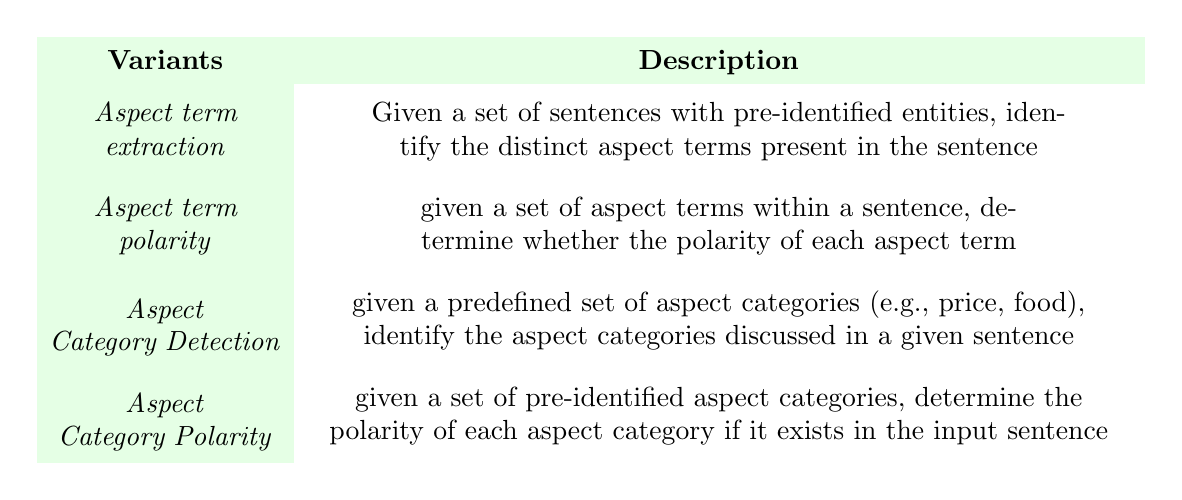
\begin{tikzpicture}
	% the matrix entries
	\matrix (mat) [table]
	{
		\textbf{Variants} & \textbf{Description} \\
		\textit{Aspect term extraction}& Given a set of sentences with pre-identified entities, identify the distinct aspect terms present in the sentence \\
		\textit{Aspect term polarity} & given a set of aspect terms within a sentence, determine whether the polarity of each aspect term \\
		\raisebox{-5mm}{\shortstack{\textit{Aspect}\\ \textit{Category Detection}}} & given a predefined set of aspect categories (e.g., price, food), identify the aspect categories discussed in a given sentence \\
		\raisebox{-5mm}{\shortstack{\textit{Aspect}\\ \textit{Category Polarity}}} & given a set of pre-identified aspect categories, determine the polarity of each aspect category if it exists in the input sentence \\
	};
	\end{tikzpicture}
	\captionof{table}{Subtasks and variants of ABSA. Typically, the polarity categories are \{\texttt{positive, negative, neutral, conflict}\} where conflict denotes both positive and negative sentiment being expressed simultaneously} \label{table:background:absasubtasks}
\end{center}	

Task 4 of the SemEval-2014 Workshop focuses on this task, for which there are 4 subtasks (relating to the variants described Table \ref{table:background:absasubtasks}).  We focus specifically on Subtask 4 i.e. given a set of known, fixed aspects $\mathcal{A}$, and a set of fixed sentiment criterion classes $\mathcal{C}$: for each sentence $x$ in the dataset, of which aspects $\mathcal{A}' \subseteq \mathcal{A}$ appear, classify each $a_x \in \mathcal{A}'$ with one sentiment class $c(a_x) \in \mathcal{C}$. We focus on the restaurant dataset\footnote{motivated by tits similarity to the type of data the company works on - see Appendix \ref{appendix:streetbees}} which has:
\begin{gather*}
\mathcal{A} = \{ \texttt{food, service, price, ambience, anecdotes/miscellaneous}\} \\
\mathcal{C} = \{ \texttt{positive, negative, neutral, conflict, none}\}
\end{gather*}

At the time the challenge was released (2014, prior to all advanced language modelling discussions in Section \ref{section:background:LMs}), the champion model was using crafted features based on specifically constructed lexicon features from various datasets, Part Of Speech (PoS) and Named Entity Recognition (NER) tagging (discussed in Section \ref{section:methodology:datasets}) and word and character level $n$-grams concatenated into a feature vector and put through a SVM model \cite{Kiritchenko2014}. This model was specifically domain adapted towards the restaurant task, and as such does not represent the scalability and generalisation capability to other tasks of language models such as BERT and XLNet. Nonetheless, this model outperformed all other approaches, achieving an accuracy of 82.93\% which is impressive given the task difficulty.

Recently, BERT, as discussed in Section \ref{section:background:bert}, was applied to this task but did not yield big performance increases over the traditional, custom built models like the one described above, achieving an accuracy of 83.7\% (an improvement just shy of 1\%) \cite{Sun2019}. However, the same paper proposed a novel auxilliary sentence technique whereby either auxilliary questions or pseudosentences were augmented to the input text and joint classification was performed. There were many variants of this (described in Section \ref{section:background:tabsasentenceconstruction}), but this method pushed the accuracy up to 85.9\% - a 3\% increase on the traditional custom built models.
\subsection{Sentihood - TABSA} \label{section:background:sentihood}
Target-ABSA (TABSA) generalises this notion one stage further: applying ABSA for each target entity $t$. An example from the Sentihood dataset is included in Table \ref{table:background:tabsaexample}

\begin{center}
\begin{tabular}{|c|c|c|}
	\hline
	Target & Aspect & Sentiment \\
	\hline
	{\color{black} LOCATION1} & {\color{purple} general} & {\color{green} Positive} \\
	{\color{black} LOCATION1} & {\color{cyan} price} & {\color{gray} None} \\
	{\color{black} LOCATION1} & {\color{orange} safety} & {\color{gray} None} \\
	{\color{black} LOCATION1} & {\color{pink} transit-location} & {\color{gray} None} \\
	\hline \hline
	{\color{black} LOCATION2} & {\color{purple} general} & {\color{gray} None} \\
	{\color{black} LOCATION2} & {\color{cyan} price} & {\color{red} Negative} \\
	{\color{black} LOCATION2} & {\color{orange} safety} & {\color{gray} None} \\
	{\color{black} LOCATION2} & {\color{pink} transit-location} & {\color{green} Positive} \\
	\hline
\end{tabular}
\captionof{table}{TABSA Example: {\color{black} LOCATION2} is in central London, and thus extremely expensive, whilst {\color{black} LOCATION1} is often considered the coolest area of London.} \label{table:background:tabsaexample}
\end{center}

\subsection{(T)ABSA and LMs: Auxilliary Sentence Construction Method} \label{section:background:tabsasentenceconstruction}
As eluded to in Sections \ref{section:background:semeval} and \ref{section:background:sentihood}, the current SOTA method developed this year for solving (T)ABSA style problems includes a novel (pseudo)sentence augmentation method, which researchers show strictly outperforms \textit{just} applying the language model to the problem in the multiclass classification setting \cite{Sun2019}. In this section, we detail the method, as it is integral to the thesis, and critically analyse the paper.
\begin{center}
	\resizebox{\textwidth}{!}{%
	\begin{tabular}{|c|c|c|}
		\hline
		NLI-\textbf{B} & QA-\textbf{B} & Label \\
		\hline \hline
		\textit{{\color{black} location - 1} - {\color{purple} general} - {\color{green} positive}} & \textit{is the polarity of the aspect {\color{purple} general} of {\color{black} location - 1} {\color{green} positive}?} & 1 \\
		\textit{{\color{black} location - 1} - {\color{purple} general} - {\color{red} negative}} & \textit{is the polarity of the aspect {\color{purple} general} of {\color{black} location - 1} {\color{red} negative}?} & 0 \\
		\textit{{\color{black} location - 1} - {\color{purple} general} - {\color{gray} none}} & \textit{is the polarity of the aspect {\color{purple} general} of {\color{black} location - 1} {\color{gray} none}?} & 0 \\
		\hline \hline
		\textit{{\color{black} location - 1} - {\color{cyan} price} - {\color{green} positive}} & \textit{is the polarity of the aspect {\color{cyan} price} of {\color{black} location - 1} {\color{green} positive}?} & 0 \\
		\textit{{\color{black} location - 1} - {\color{cyan} price} - {\color{red} negative}} & \textit{is the polarity of the aspect {\color{cyan} price} of {\color{black} location - 1} {\color{red} negative}?} & 0 \\
		\textit{{\color{black} location - 1} - {\color{cyan} price} - {\color{gray} none}} & \textit{is the polarity of the aspect {\color{cyan} price} of {\color{black} location - 1} {\color{gray} none}?} & 1 \\
		\hline \hline
		\textit{{\color{black} location - 1} - {\color{orange} safety} - {\color{green} positive}} & \textit{is the polarity of the aspect {\color{orange} safety} of {\color{black} location - 1} {\color{green} positive}?} & 0 \\
		\textit{{\color{black} location - 1} - {\color{orange} safety} - {\color{red} negative}} & \textit{is the polarity of the aspect {\color{orange} safety} of {\color{black} location - 1} {\color{red} negative}?} & 0 \\
		\textit{{\color{black} location - 1} - {\color{orange} safety} - {\color{gray} none}} & \textit{is the polarity of the aspect {\color{orange} safety} of {\color{black} location - 1} {\color{gray} none}?} & 1 \\
		\hline \hline
		\textit{{\color{black} location - 1} - {\color{pink} transit-location} - {\color{green} positive}} & \textit{is the polarity of the aspect {\color{pink} transit-location} of {\color{black} location - 1} {\color{green} positive}?} & 0 \\
		\textit{{\color{black} location - 1} - {\color{pink} transit-location} - {\color{red} negative}} & \textit{is the polarity of the aspect {\color{pink} transit-location} of {\color{black} location - 1} {\color{red} negative}?} & 0 \\
		\textit{{\color{black} location - 1} - {\color{pink} transit-location} - {\color{gray} none}} & \textit{is the polarity of the aspect {\color{pink} transit-location} of {\color{black} location - 1} {\color{gray} none}?} & 1 \\
		\hline \hline
		\textit{{\color{black} location - 2} - {\color{purple} general} - {\color{green} positive}} & \textit{is the polarity of the aspect {\color{purple} general} of {\color{black} location - 2} {\color{green} positive}?} & 0 \\
		\textit{{\color{black} location - 2} - {\color{purple} general} - {\color{red} negative}} & \textit{is the polarity of the aspect {\color{purple} general} of {\color{black} location - 2} {\color{red} negative}?} & 0 \\
		\textit{{\color{black} location - 2} - {\color{purple} general} - {\color{gray} none}} & \textit{is the polarity of the aspect {\color{purple} general} of {\color{black} location - 2} {\color{gray} none}?} & 1 \\
		\hline \hline
		\textit{{\color{black} location - 2} - {\color{cyan} price} - {\color{green} positive}} & \textit{is the polarity of the aspect {\color{cyan} price} of {\color{black} location - 2} {\color{green} positive}?} & 0 \\
		\textit{{\color{black} location - 2} - {\color{cyan} price} - {\color{red} negative}} & \textit{is the polarity of the aspect {\color{cyan} price} of {\color{black} location - 2} {\color{red} negative}?} & 1 \\
		\textit{{\color{black} location - 2} - {\color{cyan} price} - {\color{gray} none}} & \textit{is the polarity of the aspect {\color{cyan} price} of {\color{black} location - 2} {\color{gray} none}?} & 0 \\
		\hline \hline
		\textit{{\color{black} location - 2} - {\color{orange} safety} - {\color{green} positive}} & \textit{is the polarity of the aspect {\color{orange} safety} of {\color{black} location - 2} {\color{green} positive}?} & 0 \\
		\textit{{\color{black} location - 2} - {\color{orange} safety} - {\color{red} negative}} & \textit{is the polarity of the aspect {\color{orange} safety} of {\color{black} location - 2} {\color{red} negative}?} & 0 \\
		\textit{{\color{black} location - 2} - {\color{orange} safety} - {\color{gray} none}} & \textit{is the polarity of the aspect {\color{orange} safety} of {\color{black} location - 2} {\color{gray} none}?} & 1 \\
		\hline \hline
		\textit{{\color{black} location - 2} - {\color{pink} transit-location} - {\color{green} positive}} & \textit{is the polarity of the aspect {\color{pink} transit-location} of {\color{black} location - 2} {\color{green} positive}?} & 1 \\
		\textit{{\color{black} location - 2} - {\color{pink} transit-location} - {\color{red} negative}} & \textit{is the polarity of the aspect {\color{pink} transit-location} of {\color{black} location - 2} {\color{red} negative}?} & 0 \\
		\textit{{\color{black} location - 2} - {\color{pink} transit-location} - {\color{gray} none}} & \textit{is the polarity of the aspect {\color{pink} transit-location} of {\color{black} location - 2} {\color{gray} none}?} & 0 \\
		\hline
	\end{tabular}}
	\captionof{table}{\textbf{B}inary Auxilliary Sentence Construction Method for example in Table \ref{table:background:tabsaexample}} \label{table:background:tabsasentencesB}
	\resizebox{\textwidth}{!}{%
	\begin{tabular}{|c|c|c|}
		\hline
		NLI-\textbf{M} & QA-\textbf{M} & Label \\
		\hline
		\textit{{\color{black} location - 1} - {\color{purple} general}} & \textit{what do you think of the {\color{purple} general} of {\color{black} location - 1}?} & {\color{green} Positive} \\
		\textit{{\color{black} location - 1} - {\color{cyan} price}} & \textit{what do you think of the {\color{cyan} price} of {\color{black} location - 1}?} & {\color{gray} None} \\
		\textit{{\color{black} location - 1} - {\color{orange} safety}} & \textit{what do you think of the {\color{orange} safety} of {\color{black} location - 1}?} & {\color{gray} None} \\
		\textit{{\color{black} location - 1} - {\color{pink} transit - location}} & \textit{what do you think of the {\color{pink} transit - location} of {\color{black} location - 1}?} & {\color{gray} None} \\
		\hline \hline
		\textit{{\color{black} location - 2} - {\color{purple} general}} & \textit{what do you think of the {\color{purple} general} of {\color{black} location - 2}?} & {\color{gray} None} \\
		\textit{{\color{black} location - 2} - {\color{cyan} price}} & \textit{what do you think of the {\color{cyan} price} of {\color{black} location - 2}?} & {\color{red} Negative} \\
		\textit{{\color{black} location - 2} - {\color{orange} safety}} & \textit{what do you think of the {\color{orange} safety} of {\color{black} location - 2}?} & {\color{gray} None} \\
		\textit{{\color{black} location - 2} - {\color{pink} transit - location}} & \textit{what do you think of the {\color{pink} transit - location} of {\color{black} location - 2}?} & {\color{green} Positive} \\
		\hline
	\end{tabular}}
	\captionof{table}{\textbf{M}ultickass Auxilliary Sentence Construction Method for example in Table \ref{table:background:tabsaexample}} \label{table:background:tabsasentencesM}
\end{center}

The authors suggest the following sentence augmentation procedures outlined in Tables \ref{table:background:tabsasentencesB} and \ref{table:background:tabsasentencesM} that augment the input sentence with either a question or a pseudosentence, and have the classification be either binary or multiclass. They instantiate the pretrained BERT \cite{Devlin2018} model, and fine tune on this modified dataset to show that this procedure strictly outperforms the base case of just performing multiclass classification on the input sentences alone, conjecturing that the performance improvements from this technique leverage the models ability to perform well at NLI (and QA) tasks due to the next sentence prediction pretraining objective (discussed in Section \ref{section:background:bert}). The 4 different models achieve different top metrics on the Sentihood task, but they find on the SemEval task 4, subtask 4 (as described in Section \ref{section:background:semeval}) that the QA-\textbf{B} model achieves the highest accuracies on the SemEval dataset, as well as the highest $F_1$ score for aspects and AUC score for sentiments on the Sentihood data. We will refer to this as the TABSA ``explosion" method, as detailed in the next section.

\subsection{Analysis of the TABSA Explosion Method}
Since this method converts the (target and) aspect information into an auxilliary sentence, this is equivalent to exponentially expanding the corpus. We refer to this process as ``exploding the dataset". For a given unique input text, if there are $n_t$ target entities and $n_a$ aspects, then the datapoint is exploded into $n_t \cdot n_a$ new datapoints, where the secondary sentence that is augmented to the model determined uniqueness of the sentence pairs. On the one hand, this creates a much \textit{sparser} dataset, since many of the labels are of the null class (either `None' or 0 in the multiclass and binary cases respectively). This would almost certainly harm training if the model were learning from scratch. However, since we are initialising the language model with pretrained weights, the authors conjecture that, since BERT in particular has been trained with a next sentence prediction pretraining objective simultaneously to its Cloze task, the model is able to learn from this data since it already has some prior knowledge about NLI and QA tasks from which it can transfer learn.

The binary explosion is also interesting in the setting where the aspects are nonunique, i.e. in multilabelled data. If the aspects were instead just categories themselves, such as emotions\footnote{This is an example we will return to when looking at the industry specific dataset, cf Section \ref{section:data:streetbees}} then it could be that a person is feeling multiple emotions simultaneously. This binary approach, since the final layer is a sigmoid, will give us the probabilities of each emotion. Then, multilabel categorisation can be performed if this probability is over a certain threshold (say 0.5).

However, one drawback of this method is the computational considerations when expanding the dataset in this way. The multiclass problem means the instantiation of more parameters for each class head, but the binary explosion means much more forward passes through the model and thus a longer training time overall so there is a tradeoff.


\section{Multitask learning} \label{section:background:multitask}
In Machine Learning, we often care about optimising a particular metric of interest. In order to do this, we generally train a single model or possibly an ensemble of models that all individually try to optimise this metric to perform our desired task. We then finetune and tweak these models until their performance no longer increases. However, this might be a myopic framing of the problem; while we can generally achieve acceptable performance this way we are ignoring information that might help us do even better on the metric we care about. Specifically, this information comes from the training signals of related tasks. By sharing representations between related tasks, we can enable our model to generalise better on our original task. This is precisely the multitask learning paradigm.

One form of Multitask learning is so called \textit{continual learning} or \textit{sequential transfer learning} \cite{Parisi2018, RuderThesis} which aims to train the model with several tasks in sequence so that it remembers the previously learned tasks when learning the new ones. This method is inspired by the human learning process, since we are capable of continuously accumulating the information acquired by study or experience to efficiently develop new skills. With continual learning, the model should be able to performs well on new tasks due to the knowledge acquired during previous training. We could define transfer learning as a means to extract knowledge from a source setting and apply it to a different target setting, as demonstrated in Figure \ref{fig:background:transferlearning}.
\begin{center}
	\includegraphics[width=\textwidth]{transfer_learning_scenario.png}
	\captionof{figure}{Transfer Learning Illustration}
	\label{fig:background:transferlearning}
\end{center}

Instead of training sequentially, we could train simultaneously (or ``jointly"). Our hope is that during this joint training and optimisation of many different loss signals we will get improved generalization on our main task by leveraging the domain-specific information contained in the training signals of related tasks. We could motivate multitask learning biologically: from a pedagogical perspective, we often learn tasks first that provide us with the necessary skills to master more complex techniques. We could also motivate it in a statistical and mathematical context by viewing multitask learning as a form of \textit{inductive transfer}. Inductive transfer can help improve a model by introducing an inductive bias, which causes a model to prefer some hypotheses over others. In the case of joint multitask learning, the inductive bias is provided by the auxiliary tasks and thus acts as a form of regularisation since the model learns to prefer hypotheses that explain more than one task.

\subsection{Types of Multitask Learning}
\subsubsection{Hard Parameter Sharing}
\begin{center}
	\includegraphics[width=0.5\textwidth]{HardParameterSharing.png}
	\captionof{figure}{Hard Parameter Sharing, with image taken from \cite{Ruder2017}}
	\label{fig:background:hardparametersharing}
\end{center}

One common form of joint multitask learning is hard parameter sharing: we share hidden layers between all tasks, and have task specfic output layers and architectures ``on top" of our hidden layers which filter through to the task loss signal. This is an extremely common form for Language Modelling, and what we focus on in this thesis. The motivation is that a learned Language Model, such as those described in Section \ref{section:background:LMs}, have already in some sense ``learned language" and have a reasonable manifold on which the embeddings lie. Then, in order to perform downstream tasks, we just need simple linear layers which act as projection transformations on this space. This is shown diagramatically in Figure \ref{fig:background:hardparametersharing}

Hard parameter sharing reduces overfitting. This can be seen mathematically \cite{Baxter1997} or intuitively: the more tasks we are learning simultaneously, the more our model has to find a representation that captures all of the tasks and the less is our chance of overfitting on our original task.

\subsubsection{Soft Parameter Sharing}
\begin{center}
	\includegraphics[width=0.5\textwidth]{SoftParameterSharing.png}
	\captionof{figure}{Soft Parameter Sharing, with image taken from \cite{Ruder2017}}
	\label{fig:background:softparametersharing}
\end{center}

Another common method is soft parameter sharing: each task has its own model architecture, but the weights between each layer is ``linked" and regularised in order to encourage these parameters to have ``similar" values. This is shown in Figure \ref{fig:background:softparametersharing}. It is widely recognised that this method is infeasible for language models due to the large number of parameters, and thus duplication/scaling linearly with the number of tasks is computationally intractible.

\subsubsection{Adaption Modules}
A middle ground between the two has been explored, where additional architecture is implemented on top of the pre-existing architecture in an attempt to learn the contributions from each hidden layer and weight them appropriately. The most current SOTA review was Projected Attention Layers (PALs) in a paper titled: BERT and PALs \cite{Stickland2019}. The authors investigated a wide range of these adaption modules, including skip connections and learned layer weighting and propose an alternative attention based architecture (PALs) which use a low-dimensional multihead attention mechanism, based on the idea that it is important to include layers with inductive biases useful for the input domain. 

\subsection{Sampling Tasks} \label{section:background:samplingtasks}
A simple way to train a model on several tasks is to select a batch of training examples from each task, cycling through them in a fixed order. This is often referred to as ``round-robin" sampling, but we will refer to it as ``sequential" sampling (cf. our definitions in Section \ref{section:methodology:taskdistributions}). However, a downside to this strategy is that if each task has a different number of training examples then by the time we have seen every example from a particular task we could have looped through another, smaller tasks dataset many times. This could lead to overfitting on smaller tasks, and undertraining on larger tasks. Potentially we could alleviate this issue by manually tuning regularisation hyper-parameters for each task.
Alternatively we could employ methods where we see more examples from tasks with larger associated datasets. Concretely, we select a batch of examples from task $\tau_i$ with probability $p_{\tau_i}$ at each training step, and set $p_{\tau_i}$ proportional to $m_{\tau_i}$, the number of training examples for task $\tau_i$. This is the approach of the multi-task BiLSTM of the authors in the initial GLUE benchmark paper \cite{Wang2018}, and was used by authors in a Hierarchichal Multitask Approach for learning embeddings from semantic tasks \cite{Sanh2018} . It has the appealing property of selecting each example with the same probability as combining all the tasks and picking examples uniformly (though we train on batches from each task not single examples). This is also the approach used in BERT and PALs \cite{Stickland2019}.

What researchers found by employing these techniques, is that the final metric score does not change too much depending on the sampling schema in this setting; i.e that the sequential sampling mode is sufficient to get good improvements in the multitask learning setting. The main novel approach in this thesis is to redefine the task sampling schemas with a more biologically motivated model. The previous approach can conflate number of examples with ``difficulty of a task", since a task with more examples is sampled more. We find when considering certain datasets that this is not always the case, indeed SST-2 has 67,000 training examples but is considered quite an easy task\footnote{the reader is referred to Table \ref{table:methodology:datasets} for a breakdown of our datasets used in this thesis} and so this is almost certainly a downside of this technique. Instead, we want to employ a more reasonable strategy: sampling proportional to a hierarchichal task structure, leveraging useful subtask properties and sampling our ``main task" more frequently. The details of this methodology are deferred to Sections \ref{section:methodology:taskstructure} and \ref{section:methodology:taskdistributions}.

\subsection{Multitask learning applied to language modelling} \label{section:background:multitasklearningforLMs}
When looking at the leaderboard for the GLUE tasks \cite{Wang2018}, the best performing models on each task are actually ensemble models that are jointly trained on all of, or a subset of, the tasks. However, these tasks that the models are jointly fine tuned on are generally somewhat unrelated and this thesis proposes a different viewpoint regarding ``supporting subtasks" and optimal schemas thereof. For example, In Table 4 of the XLNet Paper \cite{Yang2019}, the authors present results of multiple settings, including single-task and multi-task, as well as single models and ensembles. In the multi-task setting, they jointly train an XLNet on the four largest datasets—MNLI, SST-2, QNLI, and QQP—and finetune the network on each of the other datasets in GLUE. Only single-task training is employed for the four large datasets to achieve the results posted. This decision is somewhat arbritrary, as described earlier.


\subsubsection{ERNIE 2.0}
The authors of ERNIE 2.0 \cite{Sun2019a} propose a way to integrate multitask learning into the pretraining of deep language models. Current pre-training procedures such as the ones in BERT \cite{Devlin2018} and XLNet \cite{Yang2019} described in Sections \ref{section:background:bert} and \ref{section:background:xlnet} usually focus on training the model with several simple tasks to grasp the co-occurrence of words or sentences. However, besides co-occurring, the authors argue that there exists other valuable lexical, syntactic and semantic information in training corpora, such as named entity, semantic closeness and discourse relation that these pretraining protocols do not fully capture. Thus, in order to extract the full lexical, syntactic and semantic information from training corpora, they propose a continual pre-training framework named ERNIE 2.0 which builds and learns incremental pretraining tasks through constant multitask learning. This methodology is outlined in \ref{fig:background:ernie}

\begin{center}
	\includegraphics[width=.75\textwidth]{ERNIE2.pdf}
	\captionof{figure}{ERNIE 2.0 Methodology \cite{Sun2019a}}
	\label{fig:background:ernie}
\end{center}

While this paper will focus on Multitask learning as a downstream task, the authors of this recent paper flip this on its head, and realise that multitask learning could instead be used to learn better word embeddings at the pretraining step. This novel idea was originally proposed in the extensions to this thesis prior to the paper being released.

The authors split the pretraining tasks into three categories: ``word-aware" tasks, ``structure-aware" tasks and ``semantic-aware" tasks. The word-aware tasks teach the model to capture the lexical information, the structure-aware tasks teach the model to capture the syntactic information of the corpus and the semantic-aware tasks prioritise the semantic signals. These tasks are represented in Figure \ref{fig:background:ernietaskstructure}, but the reader is referred to the paper \cite{Sun2019a} since the tasks are not that relevant to describe for the purposes of this thesis, but essentially expand on the dual task pretraining framework of BERT \cite{Devlin2018}.

\begin{center}
	\includegraphics[width=.9\textwidth]{ERNIE2TaskStructure.pdf}
	\captionof{figure}{ERNIE 2.0 Pretraining Task Framework \cite{Sun2019a}}
	\label{fig:background:ernietaskstructure}
\end{center}

\subsection{Multitask learning applied to ABSA}
There hasn't been much work on improving ABSA tasks using multitask learning. We propose to investigate both the classical multitask learning setting of jointly training on tasks, but also generalise this methodology in terms of jointly training via sampling tasks according to a preimposed task importance structure.

\subsection{Multitask learning for Knowledge Graph Construction}
It is clear that from the (T)ABSA methods we can construct the type of Knowledge Graphs (KGs) we motivated at the beginning of the thesis, as per Figure \ref{fig:intro:absa}. Additionally, if combined with NER tasks (or indeed other NLP tasks of interest), this type of framework could also be adapted into multitask multielement learning of the knowledge graph, in terms of the identificiation of entities and then aspect related classification of those entities. 

This knowledge graph could then be used for downstream link prediction of missing elements in the graph. An interesting and novel methodology for this, proposed by researchers at Streetbees and in proceedings for the upcoming EurNLP conference \cite{Garland2019}, proposes converting this knowledge graph into its induced grammar by creating pseudosentences that summarise the original input sentence in terms of key facts (using various weighted walk strategies over subgraphs) and using a language model to end-to-end learn this grammar. Then, link prediction just becomes next token prediction on this vocabulary of entities. However, there are much more standard graph embedding techniques capable of embedding this KG, and optionally performing link prediction \cite{Cai2017}.

\section{Meta Learning} \label{section:background:meta}
Human learning is the benchmark for intelligence, and since humans do not (tend to) learn from thousands or hundreds of thousands of examples, but instead from just a few. We would want our artificial agents to be able to do the same, learning and adapting quickly from only a few examples, and continuing to adapt as more data becomes available. This kind of fast and flexible learning is challenging, since the agent must integrate its prior experience with a small amount of new information, while avoiding overfitting to the new data. In short, we want an algorithm to learn to learn, to be able to learn structured priors from a variety of tasks and be able to apply this prior knowledge effectively on a new task on which it has limited experience of. This is precisely the goal of meta learning.

Suppose we can already solve some set of tasks $\mathcal{T} = \{\tau_1, ..., \tau_n \}$ and we are faced with some new task $\tau^*$. How do we learn it? The transfer learning and multitask learning paradigms state that we could initialise a model with the parameters of some pretrained network, and since this model has learned to solve similar tasks before it might be able to, after a bit of fine tuning, solve our new task. The meta learning framework instead approaches it from a different angle: what if we specifically set up our model training procedure to generalise between tasks? Then, when presented with a new task, since the model has been trying to optimise its generalisation capabilities and learned a set of weights that is ``close" to all of the optimal manifolds for each task \cite{Finn2017}, we still fine tune on our task but its able to generalise to the new task with a limited number of examples since it was explicitly trained to do this, unlike multitask learning.

\subsection{How we learn to learn}
In this thesis we will use a consistent notation for the meta learning terminology, which we outline in this section. Additionally, we will highlight the key changes when going from the traditional learning paradigm to the meta learning one.

In multitask learning, given a set of tasks $\mathcal{T}$, we are training the model to find a set of weights that jointly solves all tasks. In meta learning, given a set of tasks $\mathcal{T}$, we are training our model to learn a set of weights that is able to generalise from any task in $\mathcal{T}$ to any other task in $\mathcal{T}$. This is a more conservative setup and will probably not be able to perform better at each of the individual tasks in $\mathcal{T}$ compared to multitask learning, but it is able to generalise to new tasks much more effectively since that was how the model was trained.

The main difference between meta learning and regular learning is that \textit{datapoints in meta learning are datasets}. In the meta learning paradigm, we aim to improve generalisation onto new datasets (corresponding to new tasks), as opposed to individual datapoints in the regular learning paradigm. This means we shift our training and testing procedure to instead train, validate and test on (small) \textit{datasets}.  We have a support set $\mathcal{S}$ and a query set $\mathcal{Q}$. The support set is a set of meta training datapoints, which are themselves datasets of tasks. Task $\tau_i$ has associated training and testing datasets $\mathcal{D}_\text{train}^{(i)}$ and $\mathcal{D}_\text{test}^{(i)}$. The training and testing datasets will be performing $K$ shot learning, i.e learning to classify from just $K$ examples, and will thus be of size $K$. The support set and query set will be of size \texttt{meta\_train\_batch\_size} and \texttt{meta\_test\_batch\_size}, respectively.

\subsection{MAML}
We ideally want an algorithm for meta learning to be model agnostic, and this is what is proposed by Finn et al. in their Model Agnostic Meta Learning (MAML) algorithm \cite{Finn2017}. As long as the model is trained by (some variant of) Gradient Descent \textbf{ref for gradient descent}, we can use this algorithm to update the weights of our model in a way that is mathematically consistent with the type of behaviour we motivated in the previous paragraph.

In their approach, the parameters of the model are explicitly trained such that a small number of gradient steps with a small amount of training data from a new task will produce good generalization performance on that task. In order to get this behaviour, we would want the models internal representation to be broadly suitable for many tasks. Their evaluation shows that this algorithm compares favorably to state-of-the-art one-shot learning methods designed specifically for supervised classification, while using fewer parameters, but that it can also be readily applied to regression and reinforcement learning settings.

Algorithm \ref{alg:background:maml} shows the pseudocode for the MAML algorithm, and one can clearly see that it makes no \textit{a priori} assumptions on the model. There are two key components: the inner training step, which uses some setting of the base model parameters to calculate batchwise updates over tasks and the meta training step, which uses these adjusted model parameters to calculate the loss function, and take a gradient descent step in the average loss direction to update our base model parameters ready for the next inner training loop on a new batch of tasks.

\begin{algorithm}
	\caption{Model Agnostic Meta Learning (MAML) \cite{Finn2017}}
		\label{alg:background:maml}
	\begin{algorithmic}[1]
		\Require{p($\mathcal{T}$) - distribution over tasks}
		\Require{$\alpha, \beta$ - inner and outer learning rates/step sizes}
		\Require{Model $f_\theta$}
		\State {Randomly Initialise $\theta$, the model weights}
		\While{not done}
			\State {Sample batch of tasks $\mathcal{B} = \{\tau_i\} \sim p(\mathcal{T})$}
			\For{$\tau_i$ in $\mathcal{B}$}
				\State{Evaluate $\nabla_\theta \mathcal{L}_{\tau_i}(f_\theta)$ with respect to $K$ examples} \Comment{$K$ shot learning}
				\State {// \textit{Compute adapted parameters with gradient descent (inner training loop)}}
				\Let{$\theta'_i$}{$\theta - \alpha \nabla_\theta \mathcal{L}_{\tau_i}(f_\theta)$}
			\EndFor
			\State {// \textit{Compute model parameters with gradient descent (outer/meta training loop)}}
			\Let{$\theta$}{$\theta - \beta \nabla_\theta \sum \limits_{\tau_i \sim p(\mathcal{T})} \mathcal{L}_{\tau_i}(f_{\theta'_i})$}
		\EndWhile
	\end{algorithmic}
\end{algorithm}

\subsection{Reptile \& FOMAML}
The Reptile algorithm \cite{Nichol}, as described in Algorithm \ref{alg:background:reptile}, is very syntactically similar to MAML, indeed it is not surprising it is essentially equivalent to the first order version of MAML (named FOMAML) \cite{Nichol} in the sense that they optimise both the expected average gradient of the loss over tasks, bringing the model parameters towards the minimum of the ``joint training” problem and the expected average inner product of gradients of different minibatches for a given task, improving generalization, just in different ratios.
\begin{algorithm}
	\caption{Reptile \cite{Nichol}}
	\label{alg:background:reptile}
	\begin{algorithmic}[1]
		\Require{p($\mathcal{T}$) - distribution over tasks}
		\Require{$\alpha, \beta$ - inner and outer learning rates/step sizes}
		\Require{Model $f_\theta$}
		\State {Randomly Initialise $\theta$, the model weights}
		\While{not done}
		\State {Sample batch of tasks $\mathcal{B} = \{\tau_1, \dots, \tau_n\} \sim p(\mathcal{T})$}
		\For{$\tau_i$ in $\mathcal{B}$}
		\State {Compute $W_i = \text{SGD}_\alpha(\mathcal{L}_{\tau_i}, \theta, K)$} \Comment{SGD for $K$ steps on $\mathcal{L}_{\tau_i}$ ($K$ shot learning)}
		\EndFor
		\State {// \textit{Compute model parameters with gradient descent (outer/meta training loop)}}
		\Let{$\theta$}{$\theta + \beta \frac{1}{n} \sum \limits_{i=1}^{n} \left( W_i - \theta \right)$}
		\EndWhile
	\end{algorithmic}
\end{algorithm}

\subsection{Meta Learning applied to Language Modelling}
Previous work has looked at an end-to-end meta learning language modelling system which employ LSTM architectures \cite{Wolf}, since they mimic the meta learning update rules mathematically. Recent work has attempted to generalise to meta multitask learning by employing a LSTM architecture for each of the tasks \cite{Chen2018}.

The best application of meta learning in the language modelling space is when trying to generalise between languages, they utilise MAML \cite{Finn2017} for low-resource neural machine translation, learning to adapt to low-resource languages based on multilingual high-resource language tasks \cite{Gu}.

We instead propose a model that leverages the pretrained language models described in Section \ref{section:background:LMs} in order to fine tune using a meta learning procedure for a set of tasks $\mathcal{T}$ as opposed to multitask learning. This \sout{is} {\color{red} was} a novel application of meta learning to the few shot text classification regime \textbf{expand here about why we want to do this}

Unfortunately, on 27th August, a github repo\footnote{\texttt{https://github.com/zxlzr/FewShotNLP}} appeared linking to a paper published on Arxiv \cite{Yu} that essentially does this exact procedure :( - to discuss with supervisors
 
\newpage \cleardoublepage

% CHAPTER 3 - METHODOLOGY
% ------------------------------------------------
% Nomenclature list - update if needed
\nomenclature[G]{PoS}{Part of Speech}
\nomenclature[G]{$\mathcal{A}$}{A set of aspect categories for the (T)ABSA tasks}

% ------------------------------------------------

\chapter{Methodology} \label{chapter:methodology}
In this section, we outline our specific methodology for our experiments and define the problem more fully and technically, in line with the project aims outlined in Section \ref{section:intro:projectaims}.

\section{Hypothesis}
We hypothesise that models benefitting from shared related task representations will form better word embeddings for each of the downstream tasks. This is the notion of multitask learning; simultaneously solving many downstream tasks in order to improve performance on each individual task.

We further posit that performance can be improved by looking at \textit{dependent subtasks structures}, and propose to investigate how various task sampling schemas (cf. Definition \ref{def:methodology:taskdistributions}) of these dependent subtasks improves performance on the main task. In our case, the main task we are focusing on is the (T)ABSA tasks - SemEval and Sentihood - explained in Sections \ref{section:background:semeval} and \ref{section:background:sentihood} respectively. We utilise the transformation method described in Section \ref{section:background:tabsasentenceconstruction} to pass this through a language model. Jointly, we will train related subtasks and see how it affects performance.

\section{Task Setup}

\subsection{Task Structure} \label{section:methodology:taskstructure}
In order to solve the TABSA task, we would require performing an ABSA task on each target term individually, so its safe to assume that these tasks are of near equal importance. In order to solve the ABSA task, we would want a language modelling system to be proficient at the following (sub)tasks:
\begin{itemize}
	\item Understanding of sentiment $\rightarrow$ \textbf{Sentiment Analysis Task}
	\item Understanding of aspects $\rightarrow$ \textbf{Part of Speech (PoS)/Named Entity Recognition (NER) Task} from which our model can learn important coreferencing and word disambiguation knowledge from. This is also inspired from the previous SOTA, feature crafted NLP model \cite{Kiritchenko2014} which used PoS and NER features in an SVM model.
\end{itemize}
Due to the way we have set up the (T)ABSA tasks, as per Section \ref{section:background:tabsasentenceconstruction}, one could argue that the model should consider a QA or NLI subtask from which to learn. However, the authors of the auxilliary sentence augmentation technique hypothesise that the reason the BERT pretrained LM is capable of performing so well under this construction is due to the NLI next sentence prediction task during training \cite{Sun2019}. This conjecture was largely unsubstantiated or tested in the paper. We thus propose not to include such a task, but a discussion of this is deferred to Section \ref{section:extensions:subtasks}.

We want to formalise this notion of ``supporting subtasks" that we use in this thesis, and we do so mathematically in the Section \ref{section:methodology:taskdistributions}. Then, in Section \ref{section:methodology:modelsetup}, we describe how we use these notions to complete a forward pass of the multitask model. In the next section, we will discuss the datasets we use motivated by the above analysis.

\subsection{Datasets} \label{section:methodology:datasets}
As is common in the NLP literature, we refer to ``labels" as the target classes, and our models are performing multiclass classification.
\begin{center}
	\resizebox{\textwidth}{!}{%
		\begin{tabular}{c@{\qquad}cccc@{\qquad}|ccc}
			\toprule
			\multirow{2}{*}{\raisebox{-\heavyrulewidth}{Tasks (Datasets)}} & \multicolumn{4}{c}{Properties} & \multicolumn{3}{c}{Size} \\
			\cmidrule{2-8}
			& Priority & \# Labels & \# Sentiment Classes & \# Aspects & Train & Dev & Test\\
			\midrule
			TABSA$^\dagger$ (Sentihood) & Primary & 2 & 3 & 4  & 2952 & \multicolumn{2}{c}{872} \\
			ABSA$^\dagger$ (SemEval 2014)\footnotemark & Primary & 2 & 5 & 5  & 3038 & \multicolumn{2}{c}{747} \\
			Sentiment Analysis (SST-2)\footnotemark & Secondary & 2 & 2 & - & 67349 & \multicolumn{2}{c}{872} \\
			PoS (CoNLL 2003) & Secondary & 45 & - & - & 14041 & 3250 & 3453 \\
			\hline
			Sentiment Analysis (IMDB)$^*$ & Secondary & 2 & 2 & - & 19872 & 9975 & 19872 \\
			\hline
			Classification$^\dagger$ (Streetbees Data) & Primary & 2 & - & 34 & 24303 & \multicolumn{2}{c}{3097} \\
			\bottomrule
	\end{tabular}}
	\captionof{table}{Datasets used throughout this thesis, including various properties of each dataset. $^*$ denotes dataset only used for preliminary testing (cf. Section \ref{section:experiments:sentimentonly}) \newline $^\dagger$ denotes using the QA\_\textbf{B} method to create the exploded dataset as described in Table \ref{table:background:tabsasentencesB}. All sizes are given prior to the explosion of the dataset i.e the raw number of input text sentences for each dataset. In some cases, the dev set is equal to the test set, to match the reporting statistics given in various papers and since we are fixing hyperparameters as per \cite{Sun2019} so no hyperparameter tuning is required}
	\label{table:methodology:datasets}
\end{center}
\addtocounter{footnote}{-2} %We made 2 footnote marks in the table so subtract it manually and add as below
\stepcounter{footnote} \footnotetext{specifically Task 4, Subtask 4, Restaurants dataset}
\stepcounter{footnote} \footnotetext{There is an unlabelled test set of $\sim$1k datapoints, but since reporting is often done on the dev set and is so for the papers to which we are comparing to, we keep the splits despite the heavy skew in training and dev/testing sets}

Table \ref{table:methodology:datasets} shows the datasets we employ for testing. We decided to focus on the QA\_\textbf{B} ``explosion" method for several reasons:
\begin{enumerate}
	\item It was SOTA across the board for the SemEval (ABSA) task and achieved the largest $F_1$ score on aspects and AUC on Sentiment for the Sentihood (TABSA) task
	\item The Streetbees data was actually a multi-aspect classification problem, and so we needed to have a probability for each of the aspects so we could map this onto a multi aspect output.
	\item The BERT pretraining NLI objective was itself binary - it was next sentence prediction. We hypothesised that this would enable the best performance for BERT
\end{enumerate}

\subsubsection{(T)ABSA Data}
The reader is deferred to the discussion in Sections \ref{section:background:semeval}, \ref{section:background:sentihood} and \ref{section:background:tabsasentenceconstruction} for how this data was prepared, as it is equivalent to the methods utilised in the Auxilliary Construction Method paper \cite{Sun2019}. As mentioned, we focused on the QA\_\textbf{B} method for this thesis.

\subsubsection{SST-2}
The reader is deferred to Section \ref{section:background:sst2} for a more in depth discussion of this dataset. We use the standard dataset downloaded from the GLUE benchmark tasks \cite{Wang2018}.

\subsubsection{PoS}
For the PoS task, we focus on the CoNLL 2003 Dataset \cite{Tjong} which has become the benchmark for PoS and NER testing. The authors released both an English and German version, on which we focus on the English version. As is common in NLP, we refer to the corresponding ``label" which comes from a set of classes, so the goal for this dataset is multiclass classification. The dataset is best illustrated via an example:

\begin{center}
	\begin{tabular}{||c | c | c | c||} 
		\hline
		Token & PoS Label\footnotemark & Chunking Label & NER Label  \\ [0.5ex] 
		\hline\hline
		U.N. & NNP & I-NP & I-ORG\\
		official & NN & I-NP & O\\
		Ekeus & NNP & I-NP & I-PER\\
		heads & VBZ & I-VP & O\\
		for & IN & I-PP & O\\
		Baghdad & NNP & I-NP & I-LOC\\
		. & . & O & O\\
		\hline
	\end{tabular}
	\captionof{table}{An example of the tagging schemas for CoNLL 2003}
	\label{table:methodology:nerexample}
\end{center}
\footnotetext{A comprehensive list of what these labels mean can be found at \href{{https://www.ling.upenn.edu/courses/Fall_2003/ling001/penn_treebank_pos.html}}{\texttt{https://www.ling.upenn.edu/courses/Fall\_2003/ling001/penn\_treebank\_pos.html}}. However, the reader should just be aware that these symbols roughly correspond to whether or not the word is a noun, adjective, pronoun, verb etc.}

We choose to focus on the PoS task for our use case. The NER task focuses on entities such as people, locations and organisations. Since our ABSA task requires the model to understand how adjectives are related to nouns, and its only the TABSA task that really requires notions of locations (which are themselves proper nouns) we decided that it was more relevant for the model to work on a PoS task simultaneously as it would generalise better in both the ABSA and TABSA settings.


\subsubsection{Streetbees Data} \label{section:data:streetbees}
We also take the opportunity in this thesis to apply these methods on corporate data. More information about the company partnered with this thesis, and the type of work they do, can be found in Appendix \ref{appendix:streetbees}. As a brief introduction, the company conducts consumer behaviour surveys. The goal for this particular dataset was to ascertain how individuals felt emotionally when buying a product. An ontology was constructed, resulting in numerous categories. This was a multilabelled problem, since it was possible that users could be feeling several emotions simultaneously.

To improve the quality of the labels, we filter the data so that only the labels with at least 100 unique datapoints are included, thus avoiding labels with very sparse support. Figure \ref{fig:methodology:streetbeesdatahist} shows a count of unique datapoints with corresponding label categories.
\begin{center}
	\includegraphics[width=\textwidth]{streetbees_data_hist.pdf}
	\captionof{figure}{Countplot of the Streetbees Data (emotion) categories}
	\label{fig:methodology:streetbeesdatahist}
\end{center}

We prepare the data in the QA\_\textbf{B} format as per Table \ref{table:background:tabsasentencesB}, with the prepending question string \texttt{`Do you feel'} i.e we ask questions \texttt{Do you feel} $e$ \texttt{?} for emotion $e \in \mathcal{C}$ and have binary labels. Due to the sheer number of classes, we avoid the sparsity problem of the exploded dataset by including all the positive examples as well as 5 negative class samples. This enables the model to learn much better when the number of classes is large, and is in line with the ABSA explosion method in terms of the number of aspects per datapoint.

The core advantage of this binary explosion method is that it gives probability scores of each of the emotion categories, enabling us to select multi labelled output when the probability of an emotion exceeds a certain probability threshold, which we set to the natural value of 0.5.

\subsection{Task Distributions} \label{section:methodology:taskdistributions}
We begin by defining some important concepts that will be used throughout. A task is synonymous with a dataset, as per Table \ref{table:methodology:datasets}.
\begin{definition}[Sampling Distributions] \label{def:methodology:samplingdistributions}
	A sampling distribution is the probability distribution of the sample statistic. For our purposes, the sample statistic will be a single task drawn from a categorical distribution i.e get $\tau_i \in \mathcal{T} = \{\tau_1, \dots, \tau_n\}$ with $\P(t = \tau_i | \mathbf{p}, e) = p_{\tau_i}$, where $\mathbf{p} = \begin{pmatrix} p_{\tau_1}, \dots, p_{\tau_n} \end{pmatrix}$ and $e$ is our current epoch (cf. the annealing strategy in Definition \ref{def:methodology:taskdistributions}). 
	
	In an abuse of terminology, we will refer to the sequential progression through tasks (i.e $\tau_1 \rightarrow \tau_2 \rightarrow \dots \rightarrow \tau_n \rightarrow \tau_1 \rightarrow \dots$) as a sampling distribution, despite its determinism.
\end{definition}
\begin{definition}[Task Weighting] \label{def:methodology:taskweightings}
	Define the weight of a task $\tau_i$ to be $w_{\tau_i} \in \mathbb{R}$.
\end{definition}
\begin{definition}[Task Distribution] \label{def:methodology:taskdistributions}
	The task distribution is our sampling distribution over tasks. With the same notation as in Definition \ref{def:methodology:samplingdistributions}, we in general define $p_{\tau_i} = \frac{w_{\tau_i}^{\alpha_s (e)}}{\sum \limits_{k=1}^{n} w_{\tau_k}^{\alpha_s (e)}}$ for strategy $s$. The strategies we are considering are:
	\begin{enumerate}
		\item \textbf{Random:} $\alpha = 0 \Rightarrow p_{\tau_i} = \frac{1}{n}$ i.e uniformily at random sampling tasks from $\mathcal{T}$.
		\item \textbf{Prop(ortional):} $\alpha = 1 \Rightarrow p_{\tau_i} = \frac{w_{\tau_i}}{\sum \limits_{k=1}^{n} w_{\tau_k}}$ i.e sampling proportional to the task weightings in $\mathcal{T}$.
		\item \textbf{Sqrt:} $\alpha = \frac{1}{2} \Rightarrow p_{\tau_i} = \frac{w_{\tau_i}^{\frac{1}{2}}}{\sum \limits_{k=1}^{n} w_{\tau_k}^{\frac{1}{2}}}$ i.e sampling proportional to the square root of the task weightings in $\mathcal{T}$.
		\item \textbf{Square:} $\alpha = 2 \Rightarrow p_{\tau_i} = \frac{w_{\tau_i}^2}{\sum \limits_{k=1}^{n} w_{\tau_k}^2}$ i.e sampling proportional to the square of the task weightings in $\mathcal{T}$.
		\item \textbf{Anneal:} $\alpha = 1 - c\frac{e}{E},  p_{\tau_i} = \frac{w_{\tau_i}^\alpha}{{\sum \limits_{k=1}^{n} w_{\tau_k}^{\alpha}}}$ where $c$ is a chosen (fixed) annealing constant and $E$ is the maximum number of epochs we are training for. Throughout this thesis we fix $c=0.9$.
	\end{enumerate}
	Additionally, we consider the \textbf{sequential} schedule as a task distribution.
\end{definition}

\begin{remark}
	The sequential and random task distributions are independent of the defined task weightings. This is intentional, and these sampling strategies will act as a baseline on which we aim to compare results to. Traditional multitask learning is usually done sequentially, often referred to as the ``round robin strategy".
\end{remark}

A desirable property of the task weightings is that if a task $\tau_i$ is \textit{more important} than task $\tau_j$, then we would want a higher task weighting, i.e. $w_{\tau_i} > w_{\tau_j}$. An alternative viewpoint that was initially considered was the ``difficulty of the task" in terms of learning ability. One potential proxy for task difficulty is the number of training examples for each task, $m_{\tau_i}$ since it could be the case that tasks with less data are harder to learn from. However, we found (cf. Table \ref{table:methodology:datasets}) that some tasks that were considered ``easy to learn" such as SST-2 have large volumes of data and thus setting $w_{\tau_i} \propto m_{\tau_i}$ seemed unwise.

We instead opted for the following strategy: define each task $\tau \in \mathcal{T}$ to have an ``importance" attribute, which is one of \{`Primary', `Secondary', `Tertiary'\}. We then define the task weights as per Table \ref{table:methodology:taskweights}, where each successively higher tier is weighted twice as much as the previous tier. This is, of course, an arbritrary choice but it should demonstrate the idea effectively. Further discussions around this occur in Section \ref{section:extensions:taskweightings}.

\begin{center}
	\begin{tabular}{||c | c||} 
		\hline
		Importance of task $\tau$ & $w_{\tau}$  \\ [0.5ex] 
		\hline\hline
		Primary & 4 \\ 
		\hline
		Secondary & 2  \\
		\hline
		Tertiary & 1  \\
		\hline
	\end{tabular}
	\captionof{table}{The task weightings corresponding to each importance level}
	\label{table:methodology:taskweights}
\end{center}


\section{Model Architecture Setup} \label{section:methodology:modelsetup}
We instantiate a base language model, which is either BERT \cite{Devlin2018} or XLNet \cite{Yang2019}, through the \texttt{pytorch-transformers}\footnote{\href{www.github.com/huggingface/pytorch-transformers}{\texttt{www.github.com/huggingface/pytorch-transformers}}} library. We build upon this library rather substantially, however, but this allows us to access the respective embeddings from which we can use on downstream tasks. Specifically, we rewrite a lot of the data processing pipeline code and extracting features code to be cleaner and neater for our purposes, and to deal with the NER task which is not included by default, additionally formalising a standard dataset structure (in the form of a .csv read in by pandas). Then, these features are passed through the base language models as implemented in the \texttt{pytorch-transformers} library to get the embeddings. 

We build our multitask architecture as follows: for each task $\tau \in \mathcal{T}$, we create a \textit{head}, which is just a simple linear projection of the \textit{sequence summary token}, of hidden dimension $d_\text{model}$, to the number of classes for that task, $|\mathcal{C}_\tau|$, which we will refer to as $\mathcal{H}_\tau$. The motivation for this simple linear projection is that we would hope the model to learn a rather complex language manifold, on which subspaces correspond to specific downstream task structures, motivating the linear projection onto this subspace. The sequence summary token is the special classification token that is added by default to each sentence, \texttt{[CLS]} for BERT and \texttt{<cls>} for XLNet. While the library has functionality to summarise the sentence in numerous ways (such as taking the average embedding of the sentence), we kept it as the default methodology that was enacted at training time of these models.

When running a forward pass of this model, with the aim of jointly multitask learning tasks $\mathcal{T}$, we sample a batch of task $\tau$ according to a \textit{task distribution} (See definition \ref{def:methodology:taskdistributions}) and forward pass this batch through the base language model and the appropriate head $\mathcal{H}_\tau$. Then, the loss is computed and backpropagated through the entire model. The library can support both classification (via Cross Entropy Loss) and regression (via MSE Loss) tasks, but we only consider classification tasks in this thesis. Additionally, there is support in the library for the gradual unfreezing of the base language model layers, but the reader is diverted to Section \ref{section:experiments:unfreezing}.

As the number of steps per epoch that the model takes in the multitask setup is not well defined, we have several choices. Since, in this setup, we are sampling tasks randomly, there is no guarantee of going through ``every example in every task". Thus, we need a heuristic for how many steps we should take. We want this to collapse onto going through all tasks in the single task setting, and there are many choices. The one adopted for this thesis is the mean of the number of training examples for each task:
\begin{align*}
\text{\texttt{num\_steps\_per\_epoch}} = \text{\texttt{mean}} (m_{\tau_1}, \dots, m_{\tau_n})
\end{align*} 

There are many choices for such a function, and it could be the case that a median better accounts for skews in dataset size. However, we stuck with this reasonable heuristic for this thesis. A discussion of this is deferred to Section \ref{section:extensions:numstepsperepoch}.

\begin{algorithm}
	\caption{Training Loop Pseudocode}
	\label{alg:methodology:training}
	\begin{algorithmic}[1]
		\Require{$p$($\mathcal{T}$) - distribution over tasks defined by the \texttt{sampling\_mode}}
		\Require{Optimiser and linear scheduler, initialised with learning rates}
		\Require{Language Model $f_\theta$, and a training batch size \texttt{train\_bs}}
		\State {Initialise $\theta$, the model weights with pretrained values}
		\For{epoch in \texttt{num\_epochs}}
		\For{step in \texttt{num\_steps\_per\_epoch}}
		\State {Sample task from task distribution  $\tau \sim p(\mathcal{T})$}
		\State {Get batch of language model inputs $b_i$ for this task $\mathcal{B}_\tau = \{b_1, \dots, b_\texttt{train\_bs} \}$}
		\State {Pass this batch through the model, computing the loss on this batch $\mathcal{L}(f_\theta(\mathcal{B}_\tau))$}
		\State  {Backprop the loss through the model, updating the weights.}
		\State {Update learning rate scheduler and optimiser ready for next step}
		\EndFor
		\State{Report metrics at the end of each epoch}
		\EndFor
	\end{algorithmic}
\end{algorithm}

\section{Reporting} \label{section:methodology:reporting}
We create a folder with an experiment log for the set of tasks $\mathcal{T}$ when running an experiment. This experiment log includes ``key statistics" as reported in each of the papers and allows us a simplistic format for the easy comparison between tasks. Additionally, we include tensorboard reporting functionality \cite{tensorboard} as well as a \texttt{json} metrics report that includes a more granular report of a variety of metrics for reporting, should we need it. The tensorboard logs give us additional validation that the models are training well, and track a variety of metrics for each of the tasks while training. These metrics are outlined and explained in Table \ref{table:methodology:reporting}.
\begin{center}
	\resizebox{\textwidth}{!}{
	\begin{tabular}{|c|c|c|c|}
		\hline
		Task & Metric & Description & Current SOTA \\
		\hline
		SST-2 & Accuracy & (Total number correct) / (Total number of examples) & 0.968 \\
		\hline
		IMDB & Accuracy & (Total number correct) / (Total number of examples) & 0.974 \\
		\hline
		PoS & Accuracy & (Total number correct) / (Total number of examples) & - \\
		\hline
		\multirow{8}{*}{SemEval\_QA\_B$^\dagger$} & 2 Class Accuracy & The accuracy restricted to the two classes \{\texttt{positive, negative}\} & 0.956 \\
		& \multirow{2}{*}{3 Class Accuracy} & The accuracy restricted to the three classes  & \multirow{2}{*}{0.899} \\
		& & \{\texttt{positive, neutral, negative}\} & \\
		& \multirow{2}{*}{4 Class Accuracy} & The accuracy of all 4 classes \{\texttt{positive, neutral,}  & \multirow{2}{*}{0.859} \\ 
		& & \texttt{negative, conflict}\} - ignoring any aspects with no classification & \\
		& Precision & (True Positives) / (True Positives + False Positives) & 0.9315 \\
		& Recall & (True Positives) / (True Positives + False Negatives) & 0.9083 \\
		& F1\_Score & (True Positives) / (True Positives + False Negatives) & 0.9218 \\
		\hline
		\multirow{7}{*}{Sentihood\_QA\_B$^\dagger$} & \multirow{2}{*}{Strict Aspect Accuracy} & Calculates the strict accuracy of all 4 aspect categories  & \multirow{2}{*}{0.798} \\
		& & \{\texttt{General, Price, Safety, Transit-location}\} being correct for a given datum & \\
		& Sentiment AUC & The Area Under the Curve (AUC)$^\ddagger$ for the Sentiment Classes & 0.97 \\
		& Aspect AUC & The Area Under the Curve (AUC) for the Aspect Classes & 0.975 \\
		& Precision & (True Positives) / (True Positives + False Positives) & - \\
		& Recall & (True Positives) / (True Positives + False Negatives) & - \\
		& F1\_Score & (True Positives) / (True Positives + False Negatives) & 0.879 \\
	    \hline
	\end{tabular}}
	\captionof{table}{A table showing all the key metrics we will be reporting as per the literature, as well as brief description of each one and the current SOTA. \newline 
	$^\dagger$ We may refer to these tasks without the prepending ``\_QA\_B" in the thesis with the agreement there is no ambiguity among the tasks described in Section \ref{section:background:tabsasentenceconstruction} \newline
	$^\ddagger$ This metric combines the True Positive Rate (TPR) and the False Positive Rate (FPR) as plotted in the Reciever Operator Curve (ROC) into a singular metric, with 1.0 being perfection and 0.5 being roughly equivalent to random guessing. It is frequent to have ROC scores of greater than 0.95 in SOTA applications.}
    \label{table:methodology:reporting}
\end{center}

 
\newpage \cleardoublepage

% CHAPTER 4 - EXPERIMENTS
% ------------------------------------------------
% Nomenclature list - update if needed
\nomenclature[M]{$w_{\tau_i}$}{The weight of task $\tau_i \in \mathcal{T}$. The sampling distributions are proportional to this weight.}
\nomenclature[M]{$p(\mathcal{T})$}{Probability distribution over our tasks. This is our notation for our sampling schema/distribution.}

% ------------------------------------------------
\chapter{Experiments \& Results} \label{chapter:experiments}

In this section, we focus on the experiments we ran to validate or disprove our hypothesis: sampling tasks according to an importance subtask hierarchy and utilising multitask learning will improve performance over both multitask learning alone and regular fine tuning/transfer learning. The reader is referred to Section \ref{section:methodology:taskdistributions} for an outline of our sampling schemas. We begin with our core experimental results showcasing performance on the ABSA task we are interested in, and supplement this with preliminary and additional experiments that we ran. We wanted to run our experiments over various model architectures, as described in Section \ref{section:experiments:languagemodels} to additionally test the importance of the Next Sentence Prediction pretraining task, that is currently not well understood by the community, as mentioned in Section \ref{section:experiments:nlipretrainingimportance}. \textbf{Write more when done}

\section{Base Language Model Choices} \label{section:experiments:languagemodels}
As eluded to in Section \ref{section:background:LMs}, we will be utilising the current SOTA language models, namely BERT and XLNet. Due to computational considerations (see Section \ref{section:experiments:compute}), we decided to use the base language models with the fewest parameters in each case. This corresponds to models \texttt{bert-base-uncased} and \texttt{xlnet-base-cased}. The models are described in Sections \ref{section:background:bert} and \ref{section:background:xlnet} respectively, and casing is defined in Section \ref{section:background:casing}.

We hypothesised that casing would be influential to our models, since proper nouns (in the TABSA setting) and all capitals (generally reflecting ``anger" which correlates highly with negative sentiment) were present in some of our datapoint examples. However, it was infrequent and in our initial testing we found that the cased model tended to perform worse due to the slightly worse learned word representations on the open source datasets.

Additionally, we wanted to compare fully to the ABSA, BERT and XLNet papers \cite{Sun2019, Devlin2018, Yang2019}, which all used \texttt{bert-base-uncased} (for the former two) and \texttt{xlnet-base-cased} (for the latter) in their reporting. In order to demonstrate the value of this methodology, we wanted to introduce as few variants from the literature as possible.

Thus, we just consider the \texttt{bert-base-uncased} and \texttt{xlnet-based-cased} models.
\section{SemEval (ABSA) Results}
In this section we critically analyse our ABSA results, and posit meaningful hypotheses about the nature of our performances in the multitask setting that are pertinent to our main ABSA task. We plot graphs for each metric in a given task, for both models \texttt{xlnet-base-cased} and \texttt{bert-base-uncased}. We plot a baseline line in grey, which is the performance of the single task model (i.e. regular fine tuning/transfer learning), as well as the SOTA model performance in black. We aim to identify which sampling strategies correlate to good performances, as well as how each of the models perform on the various tasks.

The reader should note that on Figures \ref{fig:experiments:semevalaccs}, \ref{fig:experiments:semevalaccsrelative} and \ref{fig:experiments:semevalprf} the baseline and SOTA line should coincide for \texttt{bert-base-uncased} on the ABSA task . However, the original paper had some stochastic elements that could not be exactly recreated, so the model performance is within a very small, reasonable threshold of the paper performance. The SOTA values are as reported in the paper \cite{Sun2019}.

Figure \ref{fig:experiments:semevalaccs} shows the accuracies obtained by each model using all the multitask and sampling mode combinations with the $y$-axis corresponding to a specific accuracy metric (either 2 class, 3 class or 4 class) for the SemEval task. The reader is invited to look at Table \ref{table:methodology:reporting} for more information on each of these metrics. Figure \ref{fig:experiments:semevalaccsrelative} shows the same metrics and plots, but the $y$-axis instead corresponding to relative increase (or decrease) from the SOTA level. Figure \ref{fig:experiments:semevalprf} shows the precision, recall and $F_1$ score for the ABSA task, in the same format as the graphs previous.

\begin{figure}
	\makebox[\textwidth][c]{\includegraphics[width=1.3\textwidth]{SemEvalResults.pdf}}%
	\captionof{figure}{SemEval \{2,3,4\}-way accuracies on BERT and XLNet for our sampling modes}
	\label{fig:experiments:semevalaccs}
\end{figure}

\begin{figure}
	\makebox[\textwidth][c]{\includegraphics[width=1.3\textwidth]{SemEvalResults_relative.pdf}}%
	\captionof{figure}{SemEval \{2,3,4\}-way accuracies relative to SOTA performance on BERT and XLNet for our sampling modes}
	\label{fig:experiments:semevalaccsrelative}
\end{figure}

\begin{figure}
	\makebox[\textwidth][c]{\includegraphics[width=1.3\textwidth]{SemEvalResultsPRF.pdf}}%
	\captionof{figure}{SemEval Precision, Recall and $F_1$ Scores on BERT and XLNet for our sampling modes}
	\label{fig:experiments:semevalprf}
\end{figure}

\subsection{NLI Pretraining Task Importance} \label{section:experiments:nlipretrainingimportance}
As mentioned in Sections \ref{section:background:bert} and \ref{section:background:xlnet}, there are key differences in the pretraining procedure of each of our two language models under consideration: the next sentence prediction task. BERT was trained with this binary next sentence prediction task whereas XLNet was not. As discussed in Section \ref{section:background:tabsasentenceconstruction}, the performance for BERT on this ABSA task using this auxilliary sentence construction method was put down to its ability to leverage knowledge from its pretraining task enabling it to better fine tune at binary QA and NLI tasks.
We empirically validate this conjecture through extensive testing that was omitted from the original paper. Indeed, we show this in the results in Figure \ref{fig:experiments:semevalaccs}. We see that the baseline task performance (i.e just pretraining on SemEval\_QA\_B) on XLNet was \textit{worse} than BERT on the ABSA task using this method, despite it being a better language model than BERT on 20 ``classic" downstream tasks \cite{Yang2019}. This suggests that, since the (T)ABSA tasks are more difficult than the NLI/QA tasks in GLUE, it is important to have this NLI pretraining procedure for more difficult downstream tasks. This validates the importance of the NLI pretraining task, and was an important subpart of this investigation. We see, in spite of this, that the XLNet models are able to overcome the SOTA barriers using multitask learning with our task hierarchy.
We discuss later, in Section \ref{section:extensions:subtasks}, about how we might have been able to improve performance by additionally incorporating a NLI/QA task at test time, but this was omitted from this investigation. 

While it is true that XLNet is able to recover performance with downstream multitask learning, the benefits of incorporating a QA/NLI task are clear since BERT achieves a better initial performance, making a case for its inclusion as a pretraining task, and thus we conclude that the NLI task must have a role to play in order to better generalise to this complicated ABSA QA\_B type setup, as defined in Section \ref{section:background:tabsasentenceconstruction}. This aligns with the original papers of BERT and ERNIE 2.0 \cite{Devlin2018, Sun2019a}, but contrary to XLNet and RoBERTa \cite{Yang2019, Liu2019} (although we are using a different, more complicated downstream task than those tested in the papers). This means we can expand and give additional evidence that pretraining with additional tasks does help a models transfer learning abilities in the single task setting.

\subsection{Analysis of Results}
As mentioned in Section \ref{section:experiments:nlipretrainingimportance}, we established that the baseline performance of XLNet is worse than that of BERT, which is interesting in its own right. We see that, when utilising multitask learning, we outperform state of the art according to every accuracy metric as displayed in the tables in Section \ref{section:experiments:allsotaresults}. More importantly in terms of experimental validation of our methodology, we see from Table \ref{table:experiments:semevalresults} that all the models that beat SOTA 2 way accuracy sample according to our preimposed task hierarchy, commonly sampling proportionally rather than sequential or randomly which were our baselines. Unsurprisingly, the top results utilise the multitask representations of the sentiment task as well as the PoS task with the best performing model using the squared sampling schema. This extremises the importance of SemEval\_QA\_B over the other tasks whilst leveraging representations learned from subtasks of PoS and SST-2 as expected (which makes sense intuitively since both sentiment and PoS labelling tasks are useful in ABSA). This validates the approach and motivation we proposed in Section \ref{section:methodology:taskstructure}.

We additionally find that each of the top 5 performing models for binary classification for each of the model classes use the sampling schemas we defined in this thesis as opposed to just sequential sampling, thereby validating the importance of defining these schemas. We report relative improvements in an already high SOTA accuracy score of greater than 1\% in the best case. This can be seen in Table \ref{table:experiments:semevalresults}.

Where this multitask learning seems to improve results is in the much harsher metrics. We find that an \texttt{xlnet-base-cased} model fine tuning with tasks \{SST-2, NER, SemEval\_QA\_B\} using the square sampling schema achieves a 4 way accuracy of 0.8839, which is a 0.02 absolute improvement on this metric and an impressive 2.9\% relative increase on SOTA. It seems that these alternative representations enable the model to better classify classes with fewer labels in the dataset (since there is a severe label imbalance for the ``neutral" and ``conflict" classes), probably since the model does not overfit and learn to optimise just the two label setting, but instead favouring hypotheses that generalise well amongst all tasks (relating back to our discussion in Section \ref{section:background:multitask}, where the tasks act as regularisers for the model).

We see that, from Figure \ref{fig:experiments:semevalprf}, when considering Precision, Recall and F1 Scores, in general we see that \texttt{bert-base-uncased} actually performs better than XLNet in terms of beating the SOTA scores. We also conjecture this is due to the importance of the NLI pretraining task.

\begin{center}
	\resizebox{\textwidth}{!}{%
		\begin{tabular}{lllrll}
			\toprule
			Model Name &                                     Tasks & Sampling Mode &  Test Acc. (2 Class) & Absolute Increase to SOTA & Relative Increase to SOTA \\
			\midrule
			\multirow{5}{*}{bert-base-uncased} &         NER, SemEval\_QA\_B, Sentihood\_QA\_B &        anneal &                        0.963595 &                      0.01 &                     0.79\% \\
			&                  SST-2, NER, SemEval\_QA\_B &          sqrt &                        0.962457 &                      0.01 &                     0.68\% \\
			&  SST-2, NER, SemEval\_QA\_B, Sentihood\_QA\_B &          prop &                        0.960182 &                       0.0 &                     0.44\% \\
			&                       SST-2, SemEval\_QA\_B &          prop &                        0.959044 &                       0.0 &                     0.32\% \\
			&       SST-2, SemEval\_QA\_B, Sentihood\_QA\_B &          prop &                        0.959044 &                       0.0 &                     0.32\% \\
			\hline
			\multirow{5}{*}{xlnet-base-cased}  &                  SST-2, NER, SemEval\_QA\_B &        square &                        0.965870 &                      0.01 &                     1.03\% \\
			&                  SST-2, NER, SemEval\_QA\_B &        anneal &                        0.962457 &                      0.01 &                     0.68\% \\
			&       SST-2, SemEval\_QA\_B, Sentihood\_QA\_B &        anneal &                        0.961320 &                      0.01 &                     0.56\% \\
			&                  SST-2, NER, SemEval\_QA\_B &          prop &                        0.959044 &                       0.0 &                     0.32\% \\
			&       SST-2, SemEval\_QA\_B, Sentihood\_QA\_B &          prop &                        0.959044 &                       0.0 &                     0.32\% \\
			\bottomrule
	\end{tabular}}
	\captionof{table}{SemEval\_QA\_B 2 way (binary) accuracy results (restricted to the top 5 of each model that beat SOTA performance)}
	\label{table:experiments:semevalresults}
\end{center}


\section{An Overview of SOTA Results Achieved}
\label{section:experiments:allsotaresults}
\begin{center}
	\resizebox{\textwidth}{!}{
	\begin{tabular}{c@{\qquad}cccc@{\qquad}}
		\toprule
		\multirow{2}{*}{\raisebox{-\heavyrulewidth}{Metric}} & \multicolumn{4}{c}{SemEval\_QA\_B}\\
		\cmidrule{2-5}
		& Previous SOTA & Our SOTA & Model Name & Tasks (Sampling Mode) \\
		\midrule
		F1\_Score                         &        0.9218 &              0.922926 &       BERT & SST-2, SemEval\_QA\_B (random) \\
		Precision                        &        0.9315 &              0.938071 &         BERT & SST-2, SemEval\_QA\_B (prop) \\
		Recall                           &        0.9083 &              0.917073 &       BERT & SST-2, SemEval\_QA\_B (random) \\
		2 Class Accuracy  &        0.9560 &               0.96587 &  XLNet & SST-2, NER, SemEval\_QA\_B (square) \\
		3 Class Accuracy   &        0.8990 &              0.920863 &  XLNet & SST-2, NER, SemEval\_QA\_B (square) \\
		4 Class Accuracy   &        0.8590 &              0.883902 &  XLNet & SST-2, NER, SemEval\_QA\_B (square) \\
		\bottomrule
	\end{tabular}}
	\resizebox{\textwidth}{!}{
		\begin{tabular}{c@{\qquad}cccc@{\qquad}}
			\toprule
			\multirow{2}{*}{\raisebox{-\heavyrulewidth}{Metric}} & \multicolumn{4}{c}{Sentihood\_QA\_B}\\
			\cmidrule{2-5}
			& Previous SOTA & Our SOTA &Champion Model & Tasks (Sampling Mode) \\
			\midrule
			F1\_ Score & 0.879 &                0.928814 & XLNet &       SST-2, SemEval\_QA\_B, Sentihood\_QA\_B (prop) \\
			Aspect AUC           &           0.975 &                0.978023 &                      XLNet & SST-2, Sentihood\_QA\_B (sqrt) \\
			Sentiment AUC          &           0.970 &                0.973881 &  XLNet & SST-2, SemEval\_QA\_B, Sentihood\_QA\_B (sequential) \\
			Strict Aspect Accuracy  &           0.798 &                0.876201 &                      XLNet & SST-2, Sentihood\_QA\_B (prop) \\
			\bottomrule
	\end{tabular}}
	\captionof{table}{SOTA results for the TABSA tasks: SemEval and Sentihood}
	\label{table:experiments:sotaresults}
\end{center}

We see that on the TABSA and ABSA task, of which there are 10 key metrics, 7 out of 10 (70\%) of our champion models utilise our task hierarchy sampling schemas, with the most popular being square and proportional.

We see that, whilst improvements do come from the newer model (XLNet vs BERT), multitask learning further improves the previous SOTA scores, and sampling using our sampling schemas improves it even more. It is a combination of these three aspects that boosts our SOTA scores up to the levels reported in Table \ref{table:experiments:sotaresults}, particularly on Sentihood (TABSA). The graphs for the TABSA dataset are not discussed in this section, and the reader is referred to Appendix \ref{appendix:additionalfindings} for an overview of additional findings.

\section{Streetbees Results}
At an early stage in the process, we conducted this methodology using the Streetbees datasets. This was useful in testing the end to end scripts for running experiments across both models (BERT and XLNet) and a few sampling modes (we chose sequential, since it is the baseline, and prop, since it demonstrates our novel idea effectively). We did not use all sampling modes since the company was happy with a ``good" solution utilising this technology, and the models were only intended to provide as a proof-of-concept.

\subsection{Multilabel Emotion Results}
The main company dataset we will be considering is the question \textit{``How do you feel?"}, to which there is a fixed emotion set of 34 nontrivial\footnote{a label is defined as nontrivial if there was at least 100 instances of it in the entire dataset of c. 50k datapoints} labels. This data is multilabelled, thus requiring a sigmoid for each label. We thus choose to use the ABSA QA\_\textbf{B} type setup, since we get a probability of each emotion class by default since that is how the data is set up as well as the fact that these auxilliary supplementary questions mimic the way the question was asked to the users originally. The question that is augmented to the responses are \textit{``Do you feel $e$?"} for each emotion $e \in \mathcal{E}$, the set of all emotion classes.
\begin{center}
	\resizebox{\textwidth}{!}{%
		\begin{tabular}{lllrlll}
			\toprule
			& Model Name &   Tasks & Sampling Mode &  Precision & Recall & $F_1$ Score \\
			\midrule
			\multirow{2}{*}{Best Performing ($F_1$ Score)} &         \texttt{bert-base-uncased} &	SST-2, NER, SemEval\_QA\_B, Streetbees\_Mood	& prop	& 0.910938	& 0.917683	& 0.914298 \\
			&  \texttt{xlnet-base-cased}	& SST-2, Streetbees\_Mood	& prop	& 0.900042	& 0.923563	& 0.911651 \\
			\hline
			\multirow{2}{*}{Baseline (Fine tuning, single task)}  & \texttt{bert-base-uncased}	& Streetbees\_Mood	& sequential	& 0.901068	& 0.918336	& 0.909620 \\
			& \texttt{xlnet-base-cased} &	Streetbees\_Mood	& sequential	& 0.895202	& 0.926394	& 0.910531 \\
			\bottomrule
	\end{tabular}}
	\captionof{table}{Streetbees Results, showing the best performing model by $F_1$ Score compared to the baseline fine tuning models}
	\label{table:experiments:streetbeesresults}
\end{center}

The key metric that we focus on is maximising the $F_1$ Score, which is the harmonic mean of precision and recall. What we see in the results is that the best performing model for both BERT and XLNet utilise the proportional sampling scheme as opposed to ``regular" sequential multitask learning, further validating the utility of these sampling schemas. However, the baseline models still perform admirably, with the XLNet model baseline performing very similarly to the best performing one, and the BERT baseline only achieving an $F_1$ score of 0.05 less.

While the results are important, what is more useful is the impact the model has had on the business. In a presentation to the CEO, we stress tested the model. It was obviously able to match key words corresponding to the emotion categories, but more importantly it was able to do powerful inferencing steps. One standout example was the phrase \textit{``I miss my brother"}, from which the model was able to infer both sadness and loneliness categorisations; demonstrating the power of these contextualised models. Importantly from a business perspective, the marginal gains achieved by this multitask setup might be considered negligible and there is a tradeoff between good metric scores and the additional training time required for the joint multitask models to train.

The model was then additionally applied to a foodstuff ontology. A similar setup was utilised: this time the users were asked \textit{``What are you eating?"} and certain categories were identified as a labelling/coding schema such as \textit{``Chicken"} and \textit{``Wrap"} with multiple labels possible if the person was eating e.g a chicken wrap, and the responses to the questions were fed into the language models with the augmented question: \textit{``Are you eating $f$?"} for each $f$ in the food categories. This model enjoyed similar successes to the previous example, but investigations as to its efficacy are still ongoing as the company intends to incorporate image data to form a multimodal model since the text data is much noisier in this instance. This multitask multimodal system is currently being developed by researchers at the company; a component of which is the language models we have implemented for the text classification. All of the multitask language modelling frameworks have been implemented into the companies internal codebase and code reviewed.

\subsection{Generalisation Capabilities}
An interesting development from the internal conversations at the company would be how these models would generalise to a new aspect, or emotion in this case. Since the auxilliary question setup is emotion agnostic, we simply added a new emotion category to the labels: ``pride" and fed in input sentences to the model. We found that the model was only really able to ascertain exact key word matches, since it still had a learned embedding of ``pride" and was in some sense doing a similarity between the input sentence and this emotion word embedding, but it was unable to capture more nuance such as \textit{``My son just won an award"} where more inference would be required and the model has not been fine tuned to do this.

It is relatively easy for the business to label a few examples of datapoints following a new class label, such as pride, but it is unclear if the model would be able to classify them effectively in this multitask setup, since generally thousands of examples are needed (as the model performed best in practice on more common labels, as is expected). We thus turned our attention to meta learning, and explored its utility in this text classification generalisation space. We return to this idea in Section \ref{section:extensions:meta}.

\section{Preliminary Experiments}
\subsection{Ensuring Baseline Performance}
Since our architecture was much more general than typical fine tuning, and was coded from scratch but building upon a lot of various libraries, we had to ensure that in the case of a single task we recreated the performances quoted in our key literature papers. This was the first challenge. We also introduced a more stable and generalisable data ingestion format, that abstracts away a lot of the hard coded implentations for various datasets. We wrote scripts that converted each of our datasets into this standardised format and release these reformatted dataset (split) publicly.

 In particular, we focused first on recreating the SST-2 performances reported in the official BERT and XLNet papers \cite{Devlin2018, Yang2019}, since these papers were well written, with a full overview of hyperparameter choices and results, as well as the fact that the data was taken from a source that is well maintained (i.e not outdated mirror links) and is often cited. Once we recreated the performance for this, we moved on to recreating the performance quoted in the TABSA Auxilliary Sentence paper \cite{Sun2019}.

This proved more challenging, since their code was uncommented and not written for our use case. Thus, it required a lot of code rewriting and refactoring, in particular of the evaluation logic and the data formulation scripts, in order to reimplement the functionality for our purposes, as well as extending it to the more general setting we were considering. Additionally, we commented the code and abstracted various sections for open sourcing and reusability by the research community. The hyperparameters were loosely covered, and the assumption was made that all those hyperparameter settings not reported were left as the defaults in the BERT paper. With these assumptions, we were able to emulate the base performance of that in the paper.

\subsection{Gradual Unfreezing of Base Language Model Layers} \label{section:experiments:unfreezing}
As mentioned in Section \ref{section:methodology:modelsetup}, the library has support for the gradual unfreezing of the base layers. This was going to be one aspect of the multitask schema that was going to be investigated, with the hypothesis that the instantiation of the base weights provides a good initial starting point, and if we froze all layers except the final embedding layer, but as training progressed started to unfreeze deeper layers through time, we would be able to fine tune our embeddings better. We found that this was unhelpful in practice and the results were not much different from just instantiating the base model and letting gradients backpropagate through the entire model, so was omitted after this early testing stage as to not cloud the results with an unnecessary layer of complexity.

\subsection{Multitask learning for Sentiment Classification} \label{section:experiments:sentimentonly}
We began by looking at multitask learning for Sentiment Classification. In particular, we took the two most popular sentiment classification datasets: SST-2 and IMDB and tried initial experiments that would:
\begin{enumerate}[a.]
	\item Test the end to end architecture of our model on multiple tasks, and ensure the reporting was correct, as described in Section \ref{section:methodology:reporting}.
	\item Ascertain whether different tasks contributed to better learned representations and word embeddings for each seperate sentiment downstream task individually.
\end{enumerate}

These initial experiments combined the remarks in Section \ref{section:experiments:taskdistributions} with the task priorities as defined in Table \ref{table:methodology:datasets}. The results are shown in Figure \ref{fig:experiments:sentimentmultitaskresults}.

From this, we see that multitask learning does marginally improve performance on the both tasks when we use the \texttt{bert-base-uncased} model but does not yield any improvements when using the \texttt{xlnet-base-cased} model. This could be because the pretraining of XLNet was more effective at capturing word embeddings that are useful for sentiment tasks, and learning different representations in this instance does not yield any improvements. We concluded that it would not be efficient to include both tasks in our general (T)ABSA multitask learning setup and both performed similarly and, as we discuss in Section \ref{section:experiments:taskdistributions}, the number of experiments we run scaled exponentially with the number of tasks. The improvements from learning varied sentiment based word embeddings only enables the successful classification of a handful of additional examples, and thus, since two sentiment tasks seemed redundant, we decided to continue with \textit{only} the SST-2 task as a supporting sentiment task since it was the most common dataset on which sentiment analysis models are benchmarked.

\begin{center}
	\includegraphics[width=.8\textwidth]{SST2vsIMDB.pdf}
	\captionof{figure}{SST-2 vs IMDB in the single task and multitask learning setting}
	\label{fig:experiments:sentimentmultitaskresults}
\end{center}

\section{Success of the Sampling Schemas}
The previous section highlights the results of the models, showcasing the importance of a sampling schema to best leverage information from related subtasks when attempting to solve a difficult NLP task. We see that, in general, the best performing models do in fact utilise our novel sampling schema in some way, performing better than baseline multitask learning training i.e sequential (or ``round robin") task sampling. 

Unfortunately, there is no ``stand out" sampling schema. In terms of granular accuracies, the square sampling mode clearly wins on the ABSA task, and in general any type of proportional sampling gets SOTA results. The task weightings were arbritrarily defined just to showcase the idea effectively, and so a clear extension is to beter define these task weights. This is one such extension that we discuss in Section \ref{section:extensions:taskweightings}.

In general, looking at the Figures \ref{fig:experiments:semevalaccs} - \ref{fig:experiments:semevalprf} the sampling schema that often outperforms SOTA is actually the annealing strategy. This strategy is interesting, since it samples proportional to our task hierarchy initially in order to quickly learn good representations, but as the number of training steps increases the sampling schema becomes more uniform over $\mathcal{T}$; a type of smoothing process. This was motivated by the fact that early in the fine tuning process we want to take gradient descent steps using the batches of our main task and update the weights to good local minima to solve the task, but as time goes on and a good local minima is found, we want to use representations from all tasks to further refine our weights. It seems this strategy works best overall, and investigations that vary the annealing constant might prove a useful extension.

\section{Remark on Task Distributions for Experimental Optimisation} \label{section:experiments:taskdistributions}
Although it may look like when we want to run a set of experiments on tasks $\mathcal{T}$ there are:
\begin{align*}
\underbrace{2}_{\text{\#Models}} \cdot \underbrace{6}_{\#Schemas} \cdot \underbrace{\sum \limits_{r=1}^{|\mathcal{T}|} {|\mathcal{T}| \choose r}}_{=2^{|\mathcal{T}|} - 1 \text{ i.e. \# of tasks of length } r= 1,2,\dots, |\mathcal{T}|}
\end{align*}
such experiments, which scales exponentially badly, there are a few (obvious) tricks we can utilise to reduce the number of experiments, which we break down as a series of observations:
\subsubsection{Observation 1: The Single Task Setting}
In this setting, all sampling modes are equal, irrespective of the task priority. So, in this setting, we just consider the sequential schema, but really this is just normal fine tuning.

\subsubsection{Observation 2: The Two Task Setting}
\begin{prop}
	In this setting, if we have two tasks, say $\tau_i$ and $\tau_j$ of the same task priority, so that $w_{\tau_i} = w_{\tau_j}$, then the task distribution collapses onto two unique settings: the sequential (deterministic) setting, and the random setting.
\end{prop}
\begin{proof}
	For any $\alpha \in \mathbb{R}$, we have that if $w_{\tau_i} = w_{\tau_j} = w \neq 0$, say, then it follows that:
	\begin{align*}
	p_{\tau_i} = \frac{w_{\tau_i}^{\alpha}}{w_{\tau_i}^{\alpha} + w_{\tau_j}^{\alpha}} = \frac{w^{\alpha}}{w_{\tau_i}^{\alpha} + w_{\tau_j}^{\alpha}} = \frac{w_{\tau_j}^{\alpha}}{w_{\tau_i}^{\alpha} + w_{\tau_j}^{\alpha}} = p_{\tau_j}
	\end{align*}
	and so $p_{\tau_i} = p_{\tau_j} = p$ moreover that (since probabilities sum to 1), $p=\frac{1}{2}$. This can also be explicitly calculated since $p = \frac{w^{\alpha}}{w^{\alpha} + w^{\alpha}} = \frac{w^\alpha}{2w^\alpha}= \frac{1}{2}$ since $w \neq 0$.
	
	Since the sequential schema is nonrandom, it is different from the random schema, so must also be included.
\end{proof}

The proposition above enables us to eliminate the running of unneccessary experiments and sampling schemas, greatly reducing the computational time required.

\section{Training Choices} \label{section:experiments:training}
In this section, we detail the specific training choices that were made, including the hyperparameter setup and computing resources.
\subsection{Hyperparameters} \label{section:experiments:hyperparameters}
Unless otherwise stated, the experiments were all performed with hyperparameters as defaulted in the ABSA Paper \cite{Sun2019}, namely those outlined in Table \ref{table:experiments:hyperparameters}. Indeed, a thorough hyperparameter optimisation routine would have been far too computationally costly, even just over the most important hyperparameters like training batch size and learning rate. The point of this thesis was to investigate the multitask schema(s) alone, and thus fixing these hyperparameters offers a fair comparison between all schema choices. 

\begin{center}
	\begin{tabular}{||c | c||} 
		\hline
		Hyperparameter & Default Value  \\ [0.5ex] 
		\hline\hline
		Training Batch Size & 24 \\ 
		\hline
		Learning Rate & 2e-5  \\
		\hline
		Warmup Proportion & 0.1  \\
		\hline
		Number of Epochs & 4  \\
		\hline
		Annealing Constant & 0.9  \\
		\hline
		Random Seed & 42  \\
		\hline
	\end{tabular}
	\captionof{table}{The core hyperparameter default values we used throughout our testing}
	\label{table:experiments:hyperparameters}
\end{center}

Additionally, if correlates were found between optimal multitask schemas and performance improvements, hyperparameter tuning could be considered on a much smaller subset of experiments as an additional task. This is discussed in Section \ref{section:extensions:hyperparametertuning}.

\subsection{Computing Resources} \label{section:experiments:compute}
All the training was conducted on a single NVIDIA TITAN RTX GPU, named Stanley, which ran 24/7. Training of the experiments (iterating over model architecture choices as per Section \ref{section:experiments:languagemodels}, task distributions as per Section \ref{section:methodology:taskdistributions} and tasks as per Section \ref{section:methodology:datasets}) took circa 5 days, mostly owing to the large number of parameters present in the XLNet architecture.


 
\newpage \cleardoublepage

% CHAPTER 5 - EXTENSIONS
% ------------------------------------------------
% Nomenclature list - update if needed
% \nomenclature[G]{$\mathcal{D}$}{A dataset}

% ------------------------------------------------
\chapter{Extensions} \label{chapter:extensions}

In this section we propose extensions to our current study, in the form of methodological refinements, which would be quick and easy variants to the investigation we have described, then looking at methodological extensions. We also fully outline our Meta Learning strategy for Few Shot Text Classification, since we were unable to conduct any meaningful experiments due to time constraints.

\section{Methodological Refinements}

\subsection{Training Time} \label{section:extensions:numstepsperepoch}
The number of steps taken per epoch is somewhat of an arbritrary definition, indeed as is the notion of the number of epochs on which to train for. All that matters is the number of gradient descent steps we take, and ensuring that we cycle through our various tasks in a way that reasonably sees ``a good quantity" of examples from each task. We chose to do this with a sampling schema and set the number of epochs to match those used in the ABSA paper on which we intended to build upon \cite{Sun2019}. As per this paper, the metrics were reported at the end of these 4 epochs, rather than taking the best metrics achieved at some point during the 4 epochs. This means that if we configured an early stopping routine more optimally, we would have almost certainly achieved better results. The reason we chose not to was so that we could compare all of our models to the baselines in the papers, but this methodology has the unfortunate possibility of overfitting in certain cases. In the multitask setting, however, the additional tasks act as effective regularisers; introducing inductive biases into the model require the model to learn representations that satisfy all task hypotheses rather than just the single primary task. In our experimentation and inspection of the loss curves plotted, the models did not drastically overfit, and so this effect is negligible.

There is much research to be done in terms of reasonably understanding when a model should switch between subtasks and at what time in order to gain new knowledge from a different situation. Early Stopping protocols ensure the model does not overfit, but its often the case that base language models are actually underfitting, such as the case in BERT \cite{Devlin2018}.

\subsection{Subtasks} \label{section:extensions:subtasks}
Of course, the tasks we chose were motivated by the preimposed task hierarchy, but this was somewhat arbritrary - motivated only by human intuition and popular datasets that solve these tasks. We could have additionally added Question Answering (QA) and Natural Language Inference (NLI) tasks, that would almost certainly have improved the performance given the (T)ABSA sentence construction method defined in Section \ref{section:background:tabsasentenceconstruction}. However, we chose not to do this since we wanted to investigate the importance of the NLI pretraining objective (that was used in BERT, but not XLNet) on performance. Additionally, the implementational details for QA tasks are somewhat more complex, and would have been a timely procedure to implement from scratch and augment our consistent data setup with due to the inclusion of start and end span tokens in particular, but additionally adding these tasks is clearly an extension and left for the interested reader.

Another interesting experimental extension would have been to consider ``unrelated" subtasks in this context as a baseline/control case on which to judge experimental results. We felt this wasnt necessary since the single task performance metric provided a reasonable baseline from which we compared all subsequent experimental results, but it would have been interesting nonetheless and would only show to strengthen our hypothesis if the results performed worse than our selected supporting tasks for ABSA. We could hypothesise that generally multitask learning alone helps, and different latent representations produce useful downstream abilities, and the sampling schemas effect is negligible. An interesting hypothesis on which to test is how performance scales with the number of supporting tasks. On the one hand, one would expect diminishing returns as the number of tasks scale, since the optimal manifold on which we want to learn our downstream representations is shared by many of these tasks, introducing a redundency in terms of the input tasks, but it could be the case that we are still slightly underfitting and these additional tasks gradient descent the model into various regions of the parameter space on which better representations can be learned.

\subsection{Task Distributions} \label{section:extensions:taskweightings}
An interesting extensions would be if the task distribution were itself learned in some way, e.g using reinforcement learning techniques. The setup in this paper was somewhat of an arbritrary choice but provides a proof of concept for investigation. Ifthe distribution was itself learnable, one could see if the model learns to prioritise tasks in a similar way to the dsitributions we defined. However, it is possible it would not learn a meaningful distribution and just collapse onto a random structure as this is ``good enough" i.e. the model doesn't recieve a strong enough signal from the task distribution as to its relevancy, and there may be an element of hyperparameter tuning involved.

A proposal is a Reinforcement Learning type approach whereby a sampling schedule reflects how the loss decreases for each task - if it decreases the loss on the main task quite quickly then we place more emphasis on it and vice versa. This is a type of Multi Armed Bandit style setup \cite{Kuleshov2000}, where the action space is deciding which task to select a minibatch from for the next step in training.

\subsection{Hyperparameter Tuning} \label{section:extensions:hyperparametertuning}
As noted in Section \ref{section:experiments:hyperparameters}, an exhaustive grid or random hyperparameter search would have proved costly given our computational constraints, and was thus omitted from the experiments. Additionally, it is clear that hyperparameter optimisation would improve the performance but, as is common in language modelling research, the space of hyperparameters is far too large to search, and the time complexity of running these operations means only those with access to large scale distributed computing software can reasonably conduct such analyses.

As well as the hyperparameters controlling the architecture of the model, we could also vary the hyperparameters of the optimisers, or indeed the way the model summarises a sentence input (the ``sequence summary token" described in Section \ref{section:methodology:modelsetup}) to instead average the token embeddings rather than using the special classification token embedding. All of this functionality exists in the library that was built, but could not be tested over due to the computational constraints this exponentially large search would entail.

\subsection{Multiple Runs}
In our experiments, we fixed a certain random seed in which we conducted all of our experiments. Different random seeds would correspond to different task samplings and stochastic effects in the optimiser. As such, for a more rigorous study, one would want to repeat the experiments several times across several random seeds and take an average. This would make the study much more robust, but was outside the computational constraints of this study.

\section{Methodological Extensions}
\subsection{Mutual Information}
We could utilise a different approach for ABSA that would prove a very interesting extension indeed. We could investigate the role of \textit{mutual information} by introducing a hyperparameter $\lambda$ that weights the forwards and backwards information from \texttt{text\_a} (the input sentence) and \texttt{text\_b} (in the ABSA case, the corresponding pseudosentence/question asked of the input sentence as per Section \ref{section:background:tabsasentenceconstruction}). Essentially, this is like using the question to predict the response AND using the response to predict the question, and one would expect performance increases to occur if using this methodology.

\subsection{Label Smoothing}
Since neutral sentiment is a very fuzzy subjective sentimental state, training samples which are labelled neutral are unreliable. As such, we should probably employ a label smoothing regularisation term in the loss function, which penalises low entopy output distributions \cite{Szegedy}. It can reduce overfitting by preventing the network from assigning the full probability to each example in training by replacing the hard 0/1 targets with smoothed values such as 0.1 and 0.9. This trick would almost certainly improve performance, since Table \ref{table:extensions:semevalclasses} shows the distribution of sentiment classes in the ABSA Dataset is somewhat disjointed.
\begin{center}
	\begin{tabular}{c@{\qquad}ccc@{\qquad}ccc}
		\toprule
		\multirow{2}{*}{\raisebox{-\heavyrulewidth}{Dataset}} & \multicolumn{2}{c}{Positive} & \multicolumn{2}{c}{Neutral} &  \multicolumn{2}{c}{Negative} \\
		\cmidrule{2-7}
		& Train & Test & Train & Test & Train & Test\\
		\midrule
		Restaurants & 2164 & 728 & 637 & 196 & 807 & 1961 \\
		\bottomrule
	\end{tabular}
	\captionof{table}{A breakdown of the sentiment classes in the SemEval ABSA task}
	\label{table:extensions:semevalclasses}
\end{center}

\section{Meta Learning} \label{section:extensions:meta}
In terms of the flow of this thesis, we have been able to effectively build systems that leverage alternative task representations to best solve the ABSA task. We described several methodologies to improve performance on this task for use cases in academia or commercially, but we want to extend this one step further.

Given the ABSA task is quite niche in terms of large datasets, and quite granular in terms of the number of examples corresponding to a certain category, and the category classes differ from domain to domain\footnote{Indeed in the SemEval 2014 task, where we focused on Restaurant datasets, there was another dataset released that focused on Laptop reviews, where the categories were e.g battery and screen, irrelevant in the context of restaurants}, we motivate a use case for the novel application of Meta Learning to Natural Language Processing systems. The outline of the most popular and recent meta learning algorithms can be seen in Section \ref{section:background:meta}. Importantly, these algorithms are model agnostic, meaning any function that is differentiable (including our Language Models) can be used in this meta learning paradigm.

We have to set up the problem appropriately for meta learning, and in doing so we must imagine a reasonable task that we are faced with at test time. One such motivation for this work in the corporate setting was that clients often come asking how people felt about a particular category: a hot topic and the source of this example will be the category ``sustainability". This category does not exist in the dataset literature, and thus we can only hope to fine tune our model on this category. However, additionally, there is not much labelled/annotated data on this category. It is challenging to label hundreds of thousands of examples, but relatively simple to label around 100 examples. If we could design a model that is able to learn from a few examples to best predict all new incoming data, then that would solve this problem. Academically, the problem of learning complicated sentimental nuance from few examples is an interesting research problem. The hope is that the meta learning setup improves generalisation ability; the model has learned to learn from a few examples, meaning it better generalises onto the new aspect category. 

Concurrently with this thesis, this idea of few shot text classification with pre-initialised language models was independently replicated by researchers at Alibaba specifically for the case of BERT \cite{Yu}. They work on an already prepared meta learning text dataset, whereas we provide utilities to transform any dataset into this meta learning framework in our library, but report better results than applying MAML on its own to the randomly initialised language model, thereby validating the usage of language model initialisation for a ``better" starting point for training.

In our work, we use Reptile \cite{Nichol} to give a feasable methodology for training in the few shot text classification regime: For each task, which for us now is defined by a unique emotion category for the commerical dataset, or a unique aspect in the SemEval dataset, we take $K$ positive examples of this task as well as $K$ negative examples of this task. We do this for every category. Then, we construct mini datasets considering of $2K$ examples for each of the $C$ categories (e.g. $C=34$ in the case of the Streetbees Data). At training time, we perform a series of meta training steps, which consist of passing each of these mini batches of category specific datasets through the model, observing and backpropagating the loss for each category and storing all of these weight updates on each of the inner steps, then taking an outer meta training gradient descent step as per Algorithm \ref{alg:background:reptile} in Section \ref{section:background:meta}. We found in our work that the gradient update rules were fragile and possibly mathematically unstable and thus the language models did not learn effectively. A more thorough investigation of learning rates and the code would have to be conducted to continue this extension, but we provide a baseline implementation that runs end-to-end in the \texttt{TraMML} library. For more information, see Appendix \ref{appendix:code}.

\section{Knowledge Graph Extensions}
The company is currently working on a NER tagger, which is able to tag products and brands. This could be used in conjunction with the TABSA style setup: for each sentence, once targets $t$ have been identified, we could prepare auxilliary questions asking about a fixed aspect set $\mathcal{A}$ about each of the targets and build a knowledge graph using the methodology outlined in this paper. 
\newpage \cleardoublepage

\chapter{Conclusion}
The contributions of this thesis are multiple: we gave a thorough and critical investigation of multitask learning using language models, as well as defining and experimented with novel sampling schemas that mimic human task solving methodologies which provably increase performance on difficult downstream language tasks, in particular ABSA tasks. We explored how auxilliary tasks can act as effective regularisers, and touched on some important discussion regarding how the pretraining of these language models (in particular the inclusion of a NLI task) effects downstream performance. 

We conclude that sampling proportional to a subtask hierarchy is useful in achieving SOTA results on difficult downstream tasks, but these improvements are often small in terms of their relative increase. Nonetheless, in our tests 70\% of the metrics that we improved SOTA on sample proportional to the pedagogically motivated structure we defined.

Running experiments over all sampling schemas can be computationally expensive, but these sampling schemas might be useful in certain environments where the precision and/or recall of a system is important for an application, and thus every increase in these metrics is important, but the main benefits almost certainly reside in the quality of a base language model. To that end, we empirically show the importance of multitask pretraining objectives in language models, showing that despite XLNet's superiority on a range of NLP tasks such as the GLUE dataset, it fails to show the same performance increases over BERT for more complicated QA/NLI downstream tasks. Thus our recommendations are twofold: 
\begin{enumerate}
	\item The community needs a tougher benchmark for Language Model evaluation in terms of testing models on (a set of) more complicated downstream tasks
	\item The community should further research the interplay between pretraining tasks and downstream performance on related downstream tasks. A good starting point is a full ablation study of ERNIE 2.0 \cite{Sun2019a}
\end{enumerate}

We agree with the literature in that multitask fine tuning enables the model to learn better, more regularised word representations allowing it to generalise better, and contribute a well commented, scalable library for continued experimentation by the research community into Multitask and Meta Learning for Language Models: \texttt{TraMML}. We feel that this is important: the rapid rate of NLP progress leads to many new ideas being generated simultaneously, and the field would benefit from some thorough reviews and investigations into how best these transformer models learn as to direct future research. We hope this investigation provides a starting point for future work.

In terms of a corporate environment, the amount of training time required as well as time taken to build these multitask systems might offer a negligible return compared to standard transfer learning/fine tuning approaches. Thus, while our approach has proved successful, the uptake in industry for multitask systems might be slow, although useful if the upmost accuracies are required. In terms of academic contexts, this investigation provides insight into how we can manipulate the representations of language models even after pretraining to better perform at tasks, and since the idea is inspired by humanity inspired pedagogical methods this suggests that these models can benefit from learning in similar ways that humans do.

An important challenge in this space is how we generalise to new label categories, and so we outline a potential way to leverage cutting edge meta learning algorithms in order to learn more task generalisable word embeddings.

We hope that this thesis and code library provides a springboard for future research and understanding into how best these transformers learn, and the best way to pretrain and finetune these models to perform well on complicated downstream tasks, such as the ABSA tasks.

% APPENDICES
\appendix
\chapter{Streetbees: A Company Profile \& Project Relevancy}
\label{appendix:streetbees}
% Redefine header since appendix name is too long
\fancyhf{}
\fancyhead[L]{\slshape\nouppercase{Appendix A: Streetbees}}
\fancyhead[R]{\slshape\nouppercase{\thesistitle}}
\renewcommand{\headrulewidth}{0.4pt}
\fancyfoot[C]{\thepage}
%%%%%%%%%%%%%%%%%%%%%%%%%%%%%
Streetbees is a start-up focused on market research for large brands, enabling them to get ``closer" to their consumer by conducting ``in-the-moment" surveys via a conversational chatbot-like app. These surveys are either generic, or client led, and ask users questions such as ``What are you eating?" and ``What do you like about the product?". By answering these surveys the users, referred to as \textit{bees}, get financial compensation. 

The type of market research differs from traditional market research in two main ways: it asks for user feedback \textit{in the moment} i.e as they are consuming or buying the product (or immediately after), and ask about contextual factors that might motivate such a consumption or purchase; and they accept \textit{open text} responses to the questions, unlocking a potentially much richer data source than the constraints imposed by traditional multiple choice answers.

Since the company was founded in 2015, they have amassed a large dataset of close to 3 billion unique datapoints, in over 12 geographies, that capture human interaction with consumer products in the market, but also, more profoundly, form a representation of human behaviour: the underlying contextual motivating factors between purchasing decisions and buying habits. This enables them to give insights to their consumers, such as identifying previously undescovered market segmentations via clustering like the identification of a ``gamer snack" group in America - a large selection of the snack market that was previously untapped, a Streetbees survey identified the market requirement for healthy, non greasy foods compatible with gamers. 

The company intends to build a knowledge graph, representing the relationship between brands, their product portfolios and humans where the nodes are user ``logs" and the relations include links to the product (and brand) nodes mentioned in the log. Additional attributes will include how the person was feeling (sentiment) when using/consuming said product, and motivating reasons why. With attributes like this, we can perform powerful link prediction on this graph across contextual elements, contrary to the traditional demographic factor approach.

This project directly relates to the sentiment relations/nodes of the graph, and generalises the notion of how the person was feeling overall during the log to specifically. The methodologies developed in this thesis couple with this goal since it provides a robust framework for the improvement of the ABSA task, enabling knowledge graphs to be build that correctly identify user sentiment on a more granular level, specifically regarding particular aspects of products. The hope is that these models can soon generalise to entirely new, client driven, aspects as previously unseen during the training phase. This is a novel application of cutting edge NLP that is explored in this document.

The company has applied this NLP technology in a variety of applications including Mood prediction and food prediction, and is working to synergise these models with an additional vision model for images, thereby creating a multimodal image-text system. Additionally, the company is working on an NER tagger, to which we can apply the TABSA methodologies described in this paper to augment their knowledge graph functionalities in terms of understanding fine grained aspect based sentiment of user logs towards specific brands and/or their products in the way we described previously.

The meta learning framework we proposed is also of use to the company, since it aligns with a clients dynamic requirement scheme e.g. wanting to understand how users feel about new aspects of their product portfolios such as sustainability. This would mean the model would not have to be retrained from scratch, and only a minimal number of new examples would have to be labelled for the model to effectively learn this category using the structured priors it has already accumulated from previous tasks.

\chapter{Additional Findings} \label{appendix:additionalfindings}
In this section we plot some additional graphs that are not discussed in major detail in the main text. In particular, we plot the TABSA results. They are not discussed in major detail since we believe the $F_1$ score has been misreported in the literature, since we massively outperform it. In terms of the Strict Accuracy and AUC, we also beat SOTA on these metrics as referenced in Table \ref{table:experiments:sotaresults} but some of the TABSA metrics do not have reported SOTA values, so we exclude the results from our experiments section.

We exclude the plots from the supporting subtasks, since we did not achieve SOTA performance on the SST-2 task and there are no figures for the SOTA performance on the PoS CoNLL 2003 dataset (only the NER task). 
\begin{figure}
	\includegraphics[width=\textwidth]{SentihoodResults.pdf}
	\captionof{figure}{Sentihood Metric Results for Strict Accuracy, and the AUC metrics}
	\label{fig:experiments:sentihoodresults}
\end{figure}
\begin{figure}
	\includegraphics[width=\textwidth]{SentihoodResults2.pdf}
	\captionof{figure}{Sentihood Metric Results for Precision, Recall and $F_1$ Score. We believe the SOTA $F_1$ score is misreported in the literature.}
	\label{fig:experiments:sentihoodresults}
\end{figure}
\chapter{Code listings} \label{appendix:code}
We fully open source all the material in this project at:
 \begin{center}
	\href{www.github.com/RyanJenkinson/MScThesis}{\texttt{www.github.com/RyanJenkinson/MScThesis}}.
\end{center}
In this, we introduce the library \texttt{TraMML}: Transformers using Multitask and Meta Learning. We can easily use this library to normally fine tune or joint multitask fine tune onto any task by following instructions in the README of the library. It is easily configurable, by changing the \texttt{configs/run\_config.json} file that is called by \texttt{learners.py}. The quickest way to check the code implementation is to run \texttt{python learners.py} once you have installed the \texttt{requirements.txt} file.

Additionally, you can set up experiments to run by calling the \texttt{ExperimentRunner} class in \texttt{run\_experiments.py}.

Every dataset has been prepared in a consistent format, as shown in the table below. The \texttt{text\_b} column is optional, and used for the (T)ABSA tasks due to the Auxilliary Sentence Construction methodology \cite{Sun2019}. For the PoS task, the label is a list of labels.

\begin{center}
	\begin{tabular}{||c |c|c| c||} 
		\hline
		\texttt{id} & \texttt{text\_a} & \texttt{text\_b} & \texttt{label}  \\
		\hline\hline
		0 & $\vdots$ & $\vdots$ & $\vdots$ \\ 
		\hline
		1 & $\vdots$ & $\vdots$ & $\vdots$ \\ 
	\end{tabular}
	\captionof{table}{The standardised format of each input dataset as a \texttt{.csv}}
	\label{table:appendix:datasetformat}
\end{center}

To enter a new task, simply prepare the dataset in this format, add a \texttt{DataProcessor} object in \texttt{data\_processing.py} and add this to the \texttt{PROCESSORS} dictionary. Then, it is imported into the rest of the library.

\newpage
\addcontentsline{toc}{chapter}{References}
\chapter*{References}
\printbibliography[notkeyword={multitask}, notkeyword={meta}, title={General}, heading=secbib]
\printbibliography[keyword={multitask}, title={Multitask Learning}, heading=secbib]
\printbibliography[keyword={meta}, title={Meta Learning}, heading=secbib]


\end{document}